\documentclass[a4paper,12pt]{article}
\usepackage{graphicx}
\usepackage{amsmath, amssymb}
\usepackage{geometry}
\geometry{margin=1in}
\usepackage{hyperref}
\usepackage{listings}
\usepackage{xcolor}
\usepackage{float}
\usepackage{multirow}
\usepackage{array}

\title{Final Project Report: 4-bit ALU Design}
\author{Or Fachima }
\date{22/02/2025}

\begin{document}

\maketitle

\begin{abstract}
This report presents the design and implementation of a 4-bit Arithmetic Logic Unit (ALU) using Cadence Virtuoso and the gpdk045/gsclib045 technology. The ALU supports arithmetic operations, including addition and subtraction, and adheres to predefined area, timing, and voltage constraints.
\end{abstract}
\section{Introduction}
The objective of this project is to design and implement a \textbf{4-bit Arithmetic Logic Unit (ALU)} using \textbf{Cadence Virtuoso} and the \textbf{gpdk045/gsclib045} standard cell technology. The ALU performs arithmetic operations, including addition and subtraction, while adhering to predefined constraints such as \textbf{area limitations, timing requirements, and voltage levels}.

A key aspect of this project was the implementation of a \textbf{Knowles adder}, selected based on the project requirements. The Knowles adder was chosen due to its efficient parallel prefix structure, which balances speed and power consumption while maintaining reasonable layout complexity. The ALU design follows a structured approach where the addition result is stored in an internal register before subtraction is performed.

The design process was divided into two main phases:
\begin{enumerate}
    \item \textbf{Planning Stage:}
    \begin{itemize}
        \item Estimating the required standard cells.
        \item Defining the floor plan.
        \item Evaluating area constraints.
    \end{itemize}
    \item \textbf{Implementation Stage:}
    \begin{itemize}
        \item Designing the \textbf{Knowles adder} and the subtractor.
        \item Performing \textbf{detailed layout optimizations} in Virtuoso.
        \item Validating correctness through \textbf{simulations, DRC, and LVS verification}.
        \item Measuring \textbf{maximum clock frequency} under different voltage conditions.
    \end{itemize}
\end{enumerate}

The project was carried out in the \textbf{Virtuoso library} located at:  
\begin{center}
    \texttt{/project/gpdk45/users/yaishorf/ws/final\_project}
\end{center}

The following \textbf{cells contain the implementations}:
\begin{itemize}
    \item \textbf{TB} – Testbench for functional validation.
    \item \textbf{KNOWLES\_ADDER2} – Knowles adder implementation.
    \item \textbf{KNOWLES\_SUBBER1} – Subtractor implementation.
\end{itemize}

By following these structured steps, we ensured compliance with the \textbf{maximum allowable area, rise/fall time constraints, and timing requirements} as outlined in the project guidelines.
\section*{Note}
After numerous manual measurements, it became apparent that manually verifying each requirement was neither practical nor reliable. Therefore, I developed comprehensive \textbf{SKILL scripts} to systematically verify all design requirements. These scripts can be found in:

\begin{itemize}
    \item \texttt{/project/gpdk45/users/yaishorf/ws/final\_project/scripts}
\end{itemize}

Their generated reports are available in:

\begin{itemize}
    \item \texttt{/project/gpdk45/users/yaishorf/ws/final\_project/reports/}
\end{itemize}

While space limitations prevent including all these detailed measurements in this report, I would be glad to elaborate on the verification methodology and results during the project examination.

\section{Design Specifications}
\begin{itemize}
    \item \textbf{Inputs and Outputs}: A[3:0], B[3:0], C[3:0], Y[4:0].
    \item \textbf{Operations}:
    \begin{itemize}
        \item Addition: $X = A + B$
        \item Subtraction: $Y = X - C$
    \end{itemize}
    \item \textbf{Encoding}: Two’s complement representation.
    \item \textbf{Technology}: gpdk045/gsclib045.
    \item \textbf{Voltage Supply}: 1.2V.
    \item \textbf{Area Constraints}: Limited to 150\% of total cell area.
    \item \textbf{Timing Constraints}: Rise/Fall time must not exceed 50ps.
\end{itemize}
\section{Schematic Representations}
\begin{figure}[H]
    \centering
    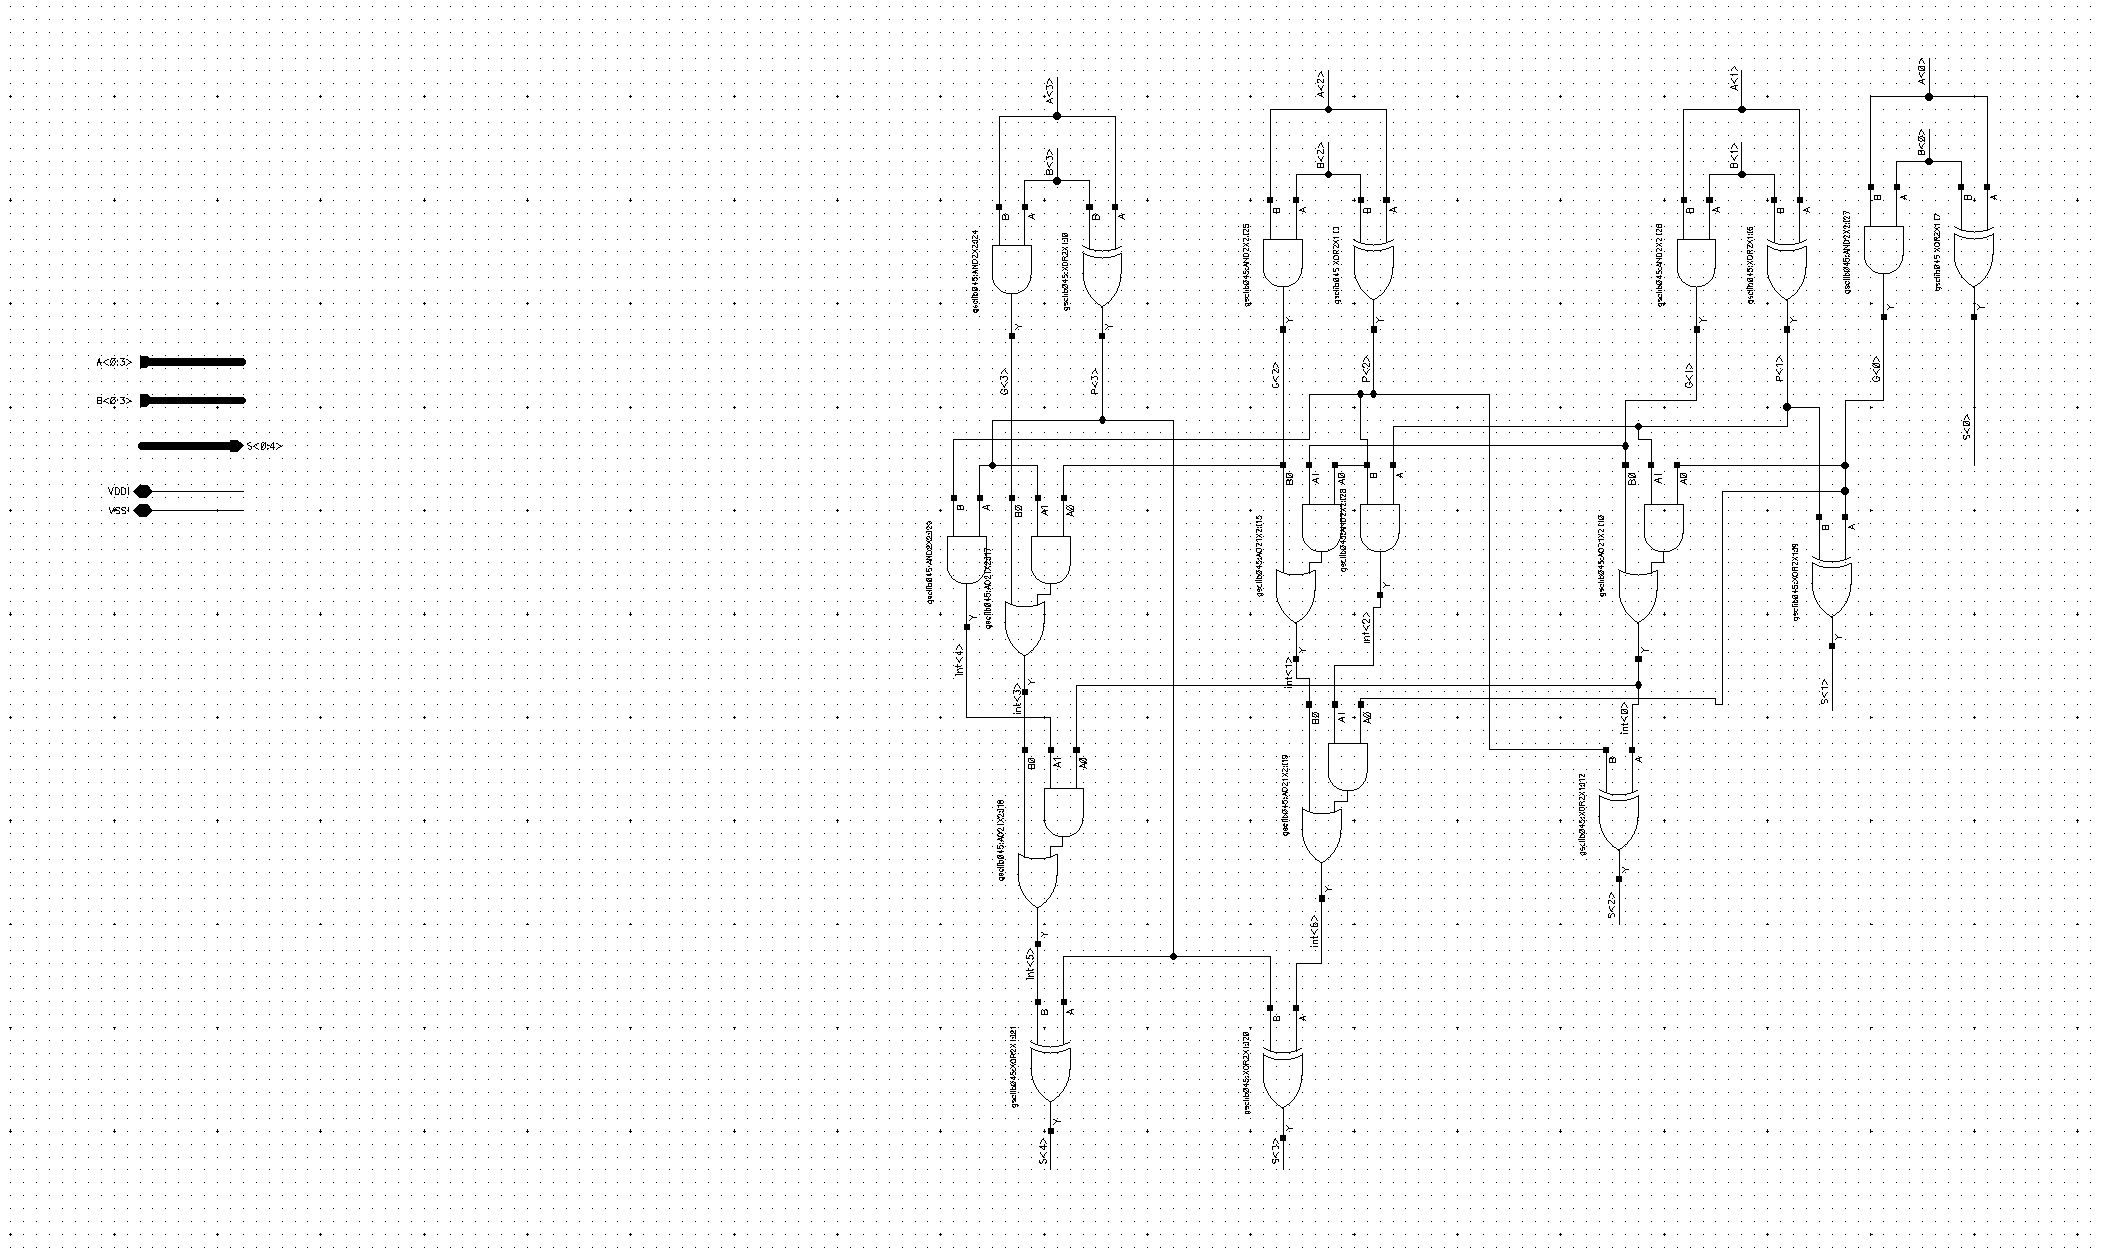
\includegraphics[width=0.8\textwidth]{images/ADD_schematic}
    \caption{Schematic of the ADD operation.}
\end{figure}

\begin{figure}[H]
    \centering
    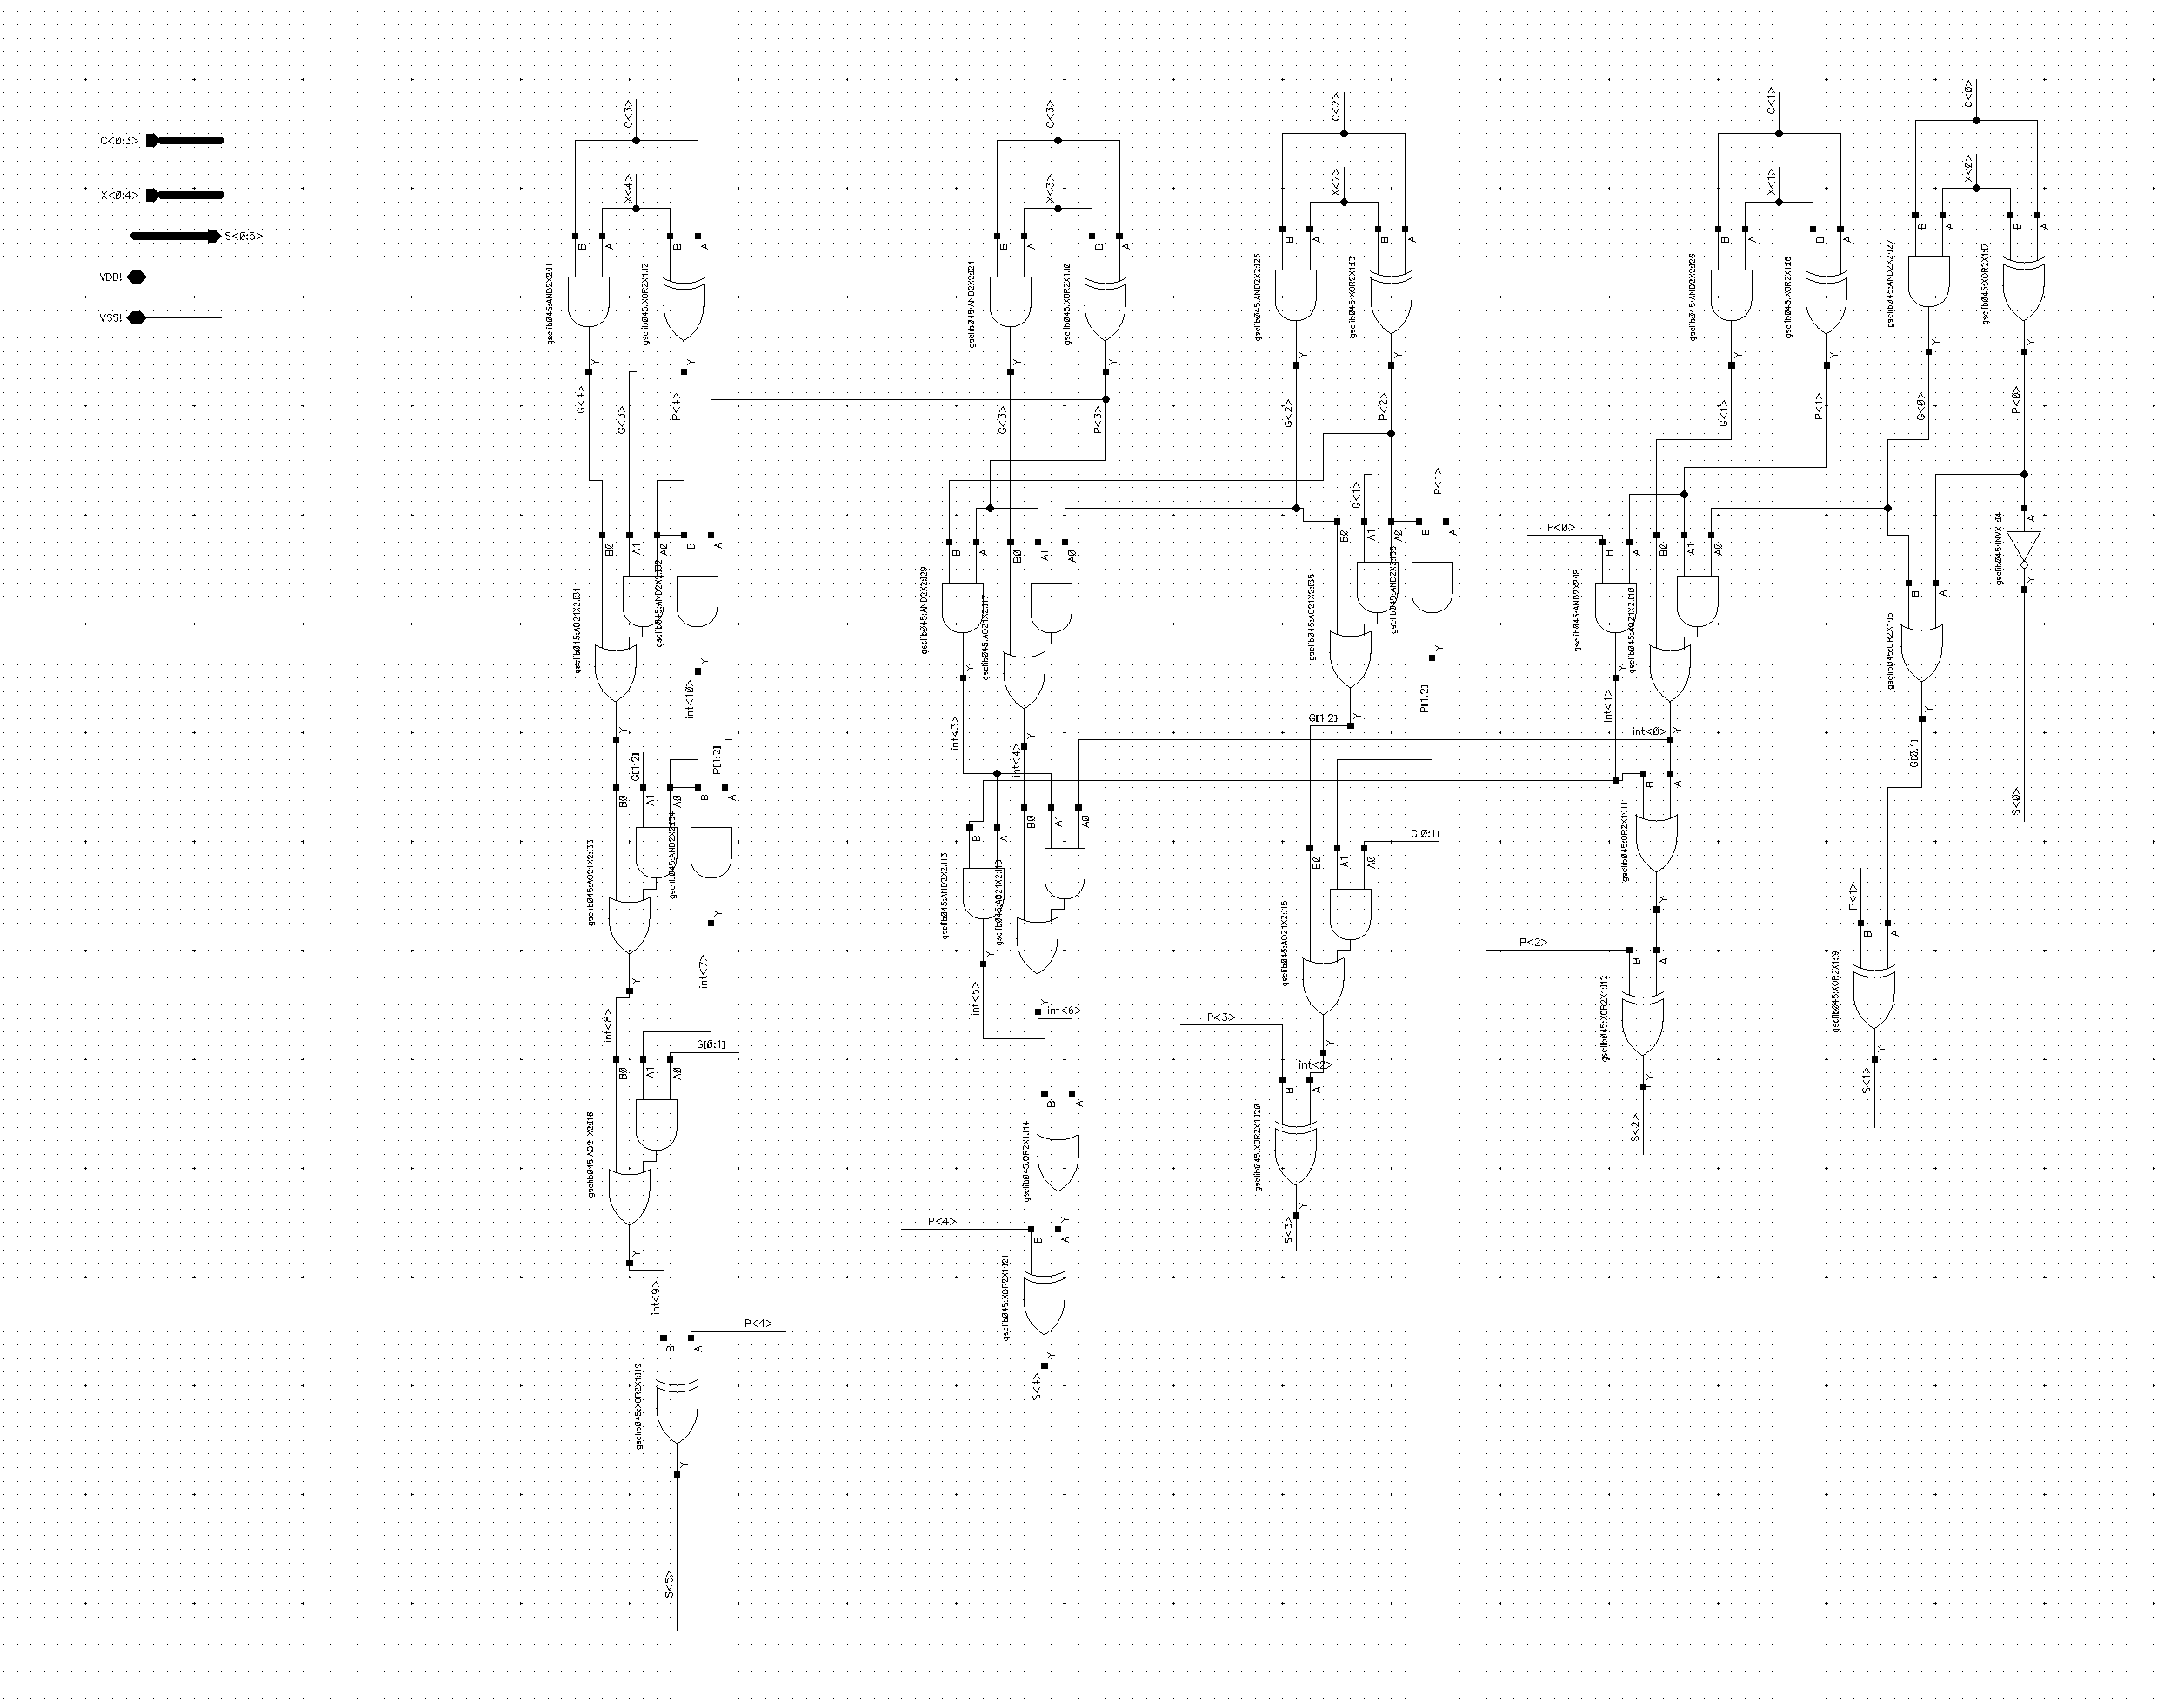
\includegraphics[width=0.8\textwidth]{images/SUB_schematic}
    \caption{Schematic of the SUB operation.}
\end{figure}

\begin{figure}[H]
    \centering
    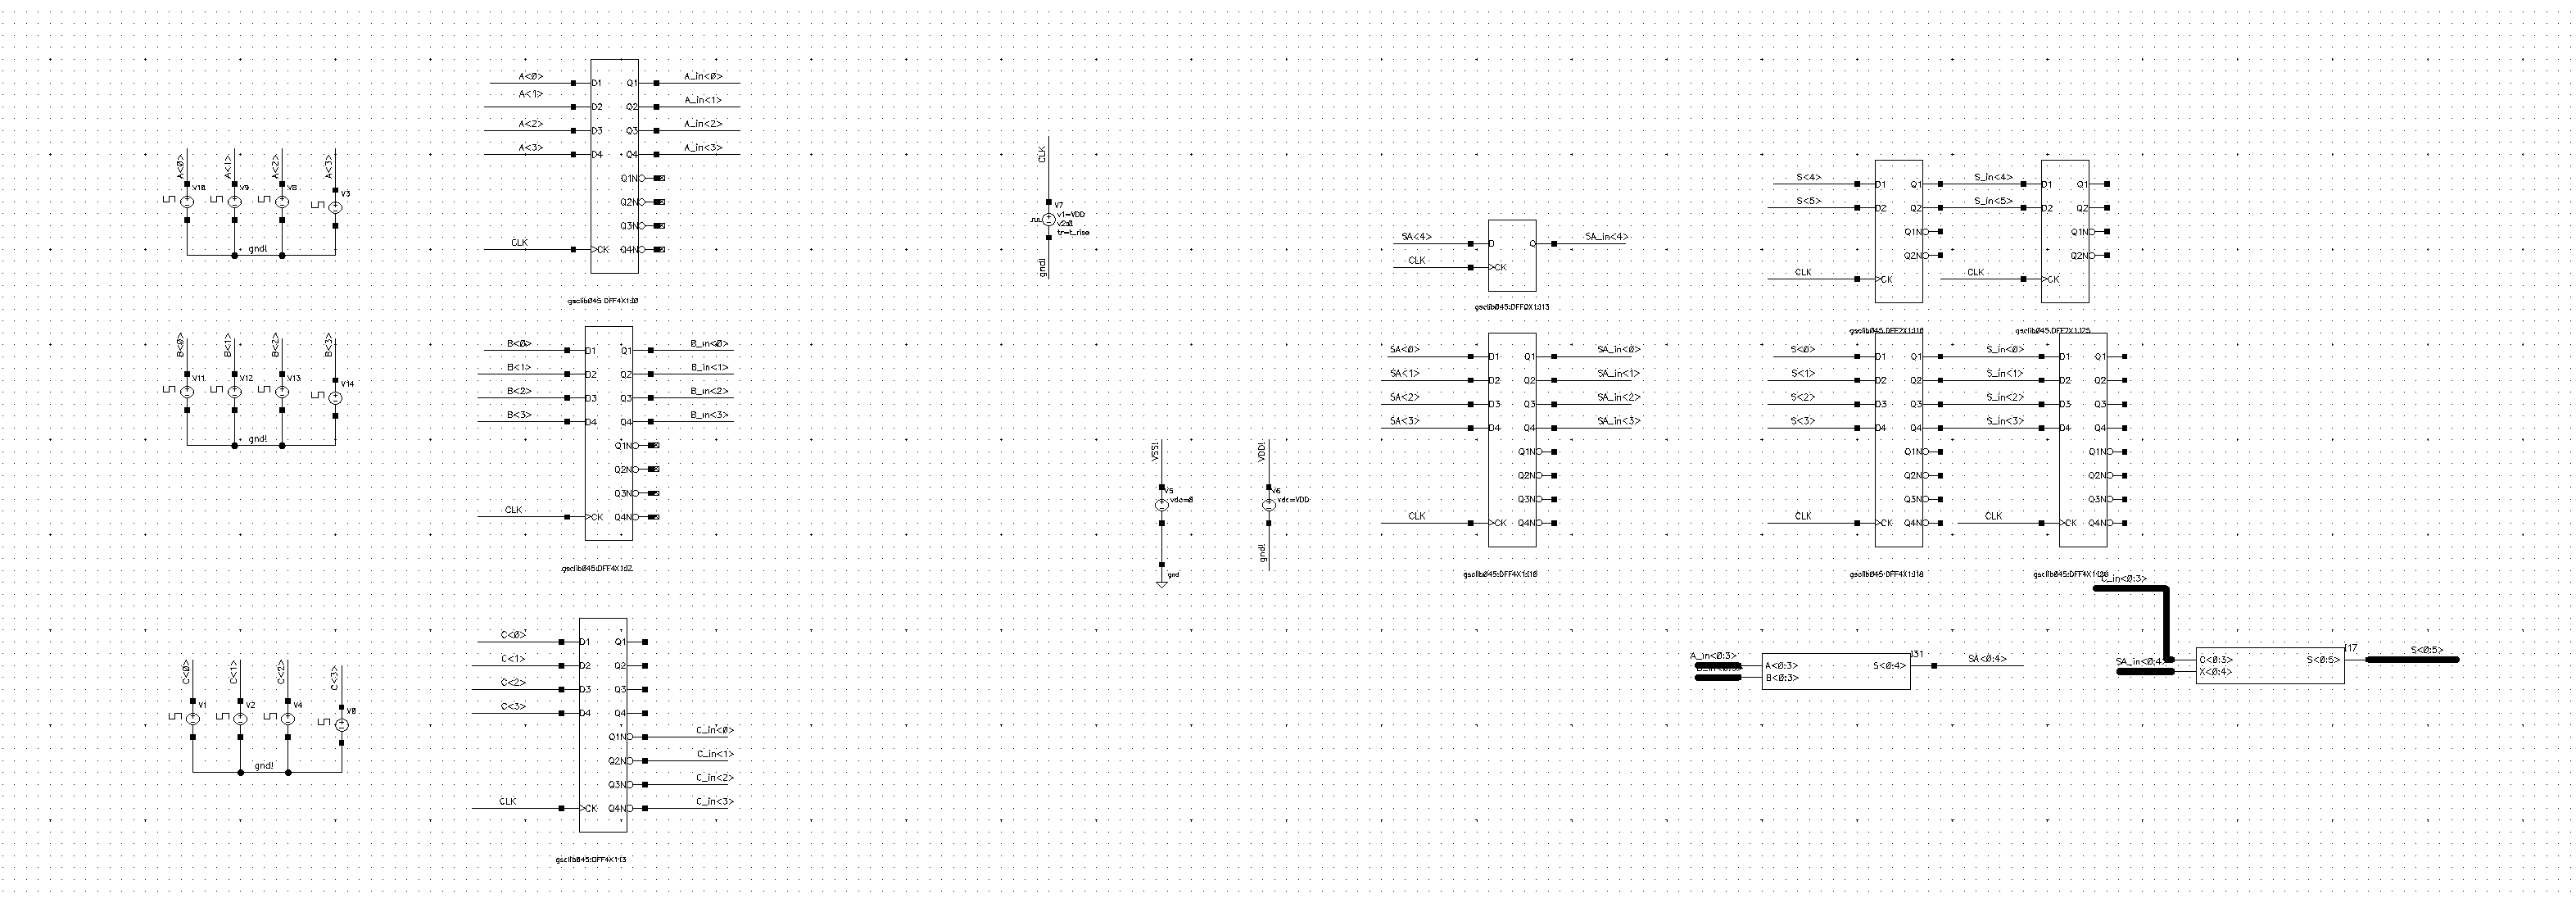
\includegraphics[width=0.8\textwidth]{images/TB_schematic}
    \caption{Testbench schematic for verification.}
\end{figure}
\subsubsection{Library Cells Used in the Design}

To design the circuit, we utilized standard cells from the \textbf{gsclib045} library. The following cells were used in different components:

\begin{itemize}
    \item \textbf{Adder:}
    \begin{itemize}
        \item 8 \texttt{XORX1}
        \item 6 \texttt{ANDX2}
        \item 5 \texttt{AOX1}
    \end{itemize}

    \item \textbf{Subtractor:}
    \begin{itemize}
        \item 10 \texttt{XORX1}
        \item 8 \texttt{ANDX2}
        \item 8 \texttt{AOX1}
        \item 2 \texttt{ORX1}
        \item 1 \texttt{INX1}
    \end{itemize}

    \item \textbf{Testbench (Sequential Elements):}
    \begin{itemize}
        \item 5 \texttt{DFF4}
        \item 1 \texttt{DFF1}
        \item 1 \texttt{DFF2}
    \end{itemize}
\end{itemize}

The use of these cells was determined based on functional requirements, power efficiency, and area constraints. The selection of flip-flops in the testbench ensured proper clocking and sequential



\section{Signal Notation}
To avoid conflicts with library cells in the simulation, the following signal conventions were used:
\begin{itemize}
    \item $<$signal\_name$>$\_in : Represents a flip-flop output.
    \item SA : Replaces X, the output of the adder.
    \item S : Replaces Y, the output of the subtractor.
\end{itemize}


\section{Implementation of the Subtractor}
The subtractor was implemented similarly to the adder, but with key modifications:
\begin{itemize}
    \item It uses the NOT of input C to perform subtraction.
    \item Modifications were made to support a default condition of $Cin = 1$.
    \item The implementation relies on the fundamental identity: $-X = \sim X + 1$.
\end{itemize}

\section{Build the Layout}

In the final implementation, we deviated slightly from the original floor plan to reduce wire lengths. It is difficult to determine whether this was the optimal decision, as layout optimization always involves trade-offs. Manual cell placement proved to be more challenging than expected, even with a relatively small number of cells. Every improvement in one wire segment often resulted in an increased wire length in another part of the design.

Throughout the process, we aimed to maintain the following design principles:
\begin{itemize}
    \item As much as possible, we kept \textbf{M2} routing vertical and \textbf{M3} routing horizontal. \textbf{M1} was barely used.
    \item Additional vias were inserted wherever feasible to reduce resistance.
    \item We tried to maintain direct wiring with minimal detours.
\end{itemize}

The following figures illustrate the final layout configuration:

\begin{figure}[H]
    \centering
    \begin{minipage}{0.49\textwidth}
        \centering
        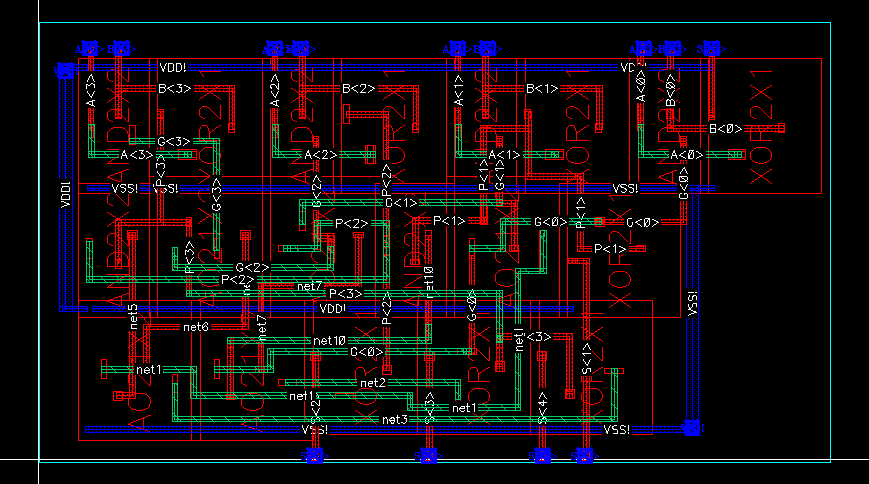
\includegraphics[width=\textwidth]{images/LO.png}
        \caption{Final Layout (View 1)}
    \end{minipage}
    \hfill
    \begin{minipage}{0.49\textwidth}
        \centering
        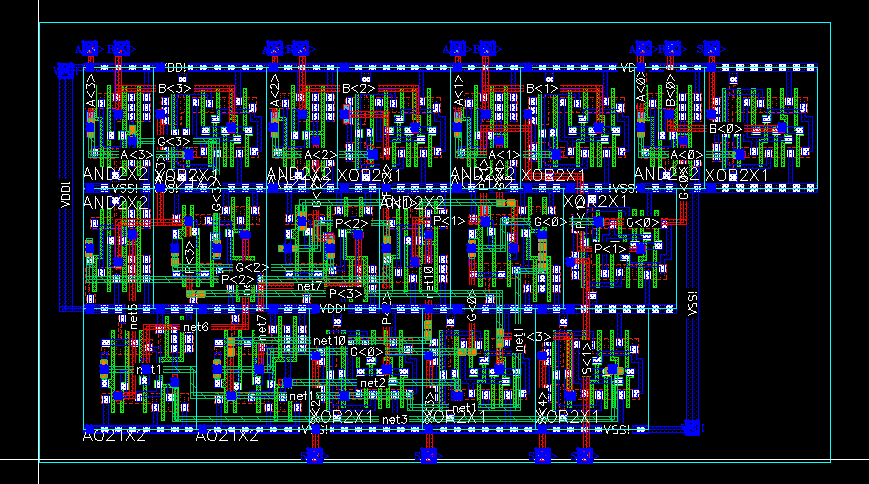
\includegraphics[width=\textwidth]{images/LO1.png}
        \caption{Final Layout (View 2)}
    \end{minipage}
\end{figure}

\begin{figure}[H]
    \centering
    \begin{minipage}{0.49\textwidth}
        \centering
        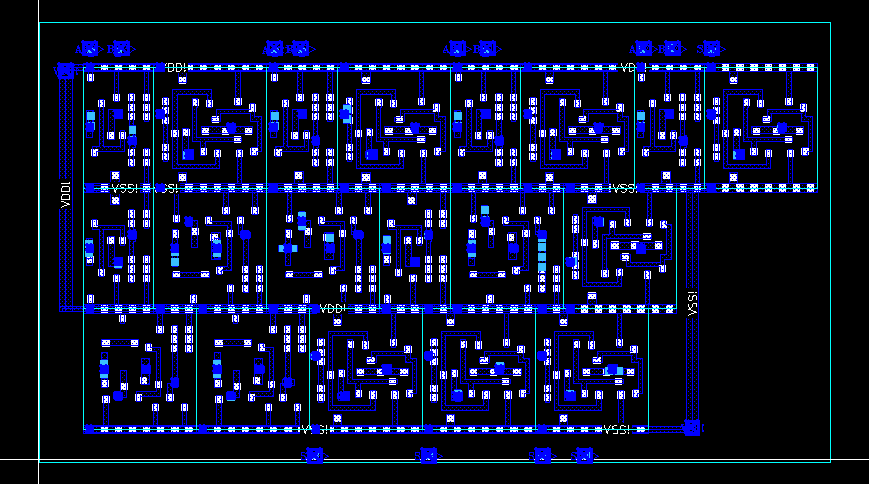
\includegraphics[width=\textwidth]{images/LO_M1.png}
        \caption{Layout Metal Layer 1 (M1)}
    \end{minipage}
    \hfill
    \begin{minipage}{0.49\textwidth}
        \centering
        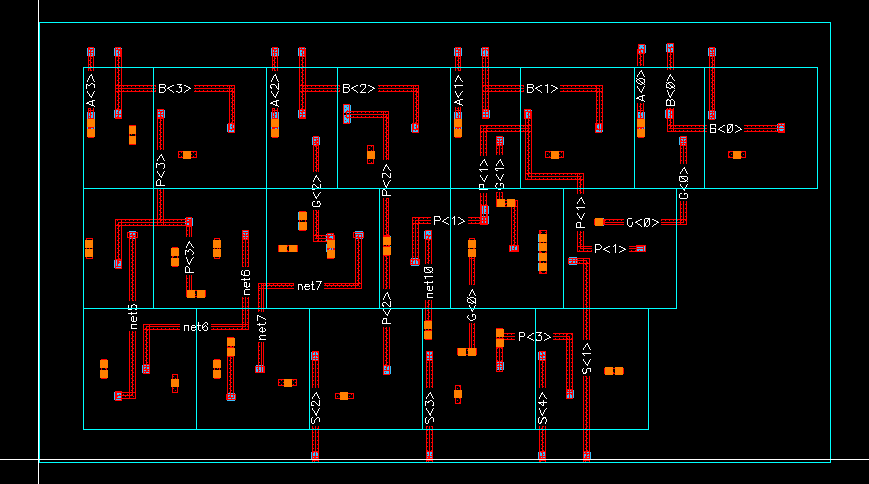
\includegraphics[width=\textwidth]{images/LO_M2.png}
        \caption{Layout Metal Layer 2 (M2)}
    \end{minipage}
    \hfill
    \begin{minipage}{0.49\textwidth}
        \centering
        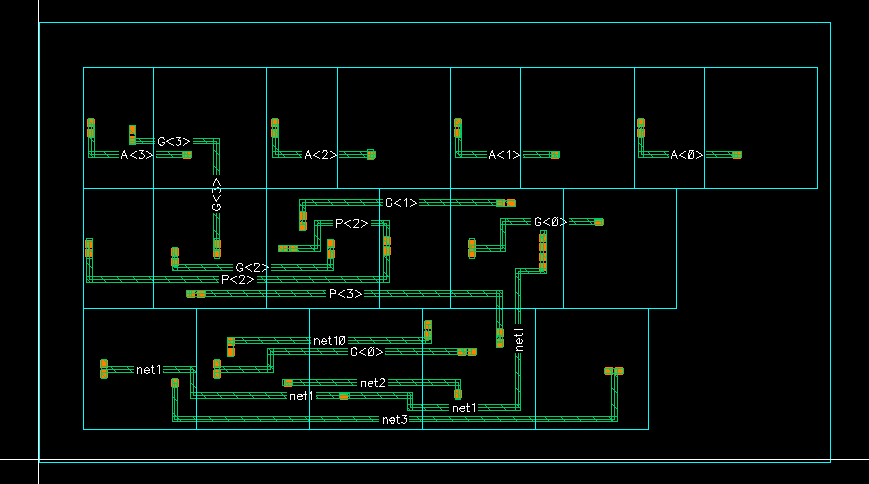
\includegraphics[width=\textwidth]{images/LO_M3.png}
        \caption{Layout Metal Layer 3 (M3)}
    \end{minipage}
\end{figure}

\subsection{Cell Area Requirement Validation}

To validate compliance with the area constraint, we performed a detailed calculation of the total cell area.

From our previous analysis, the individual cell areas were computed as follows:

\[
\text{XOR2X1 Area} = 1.9 \times 1.72 = 3.268 \, \mu m^2
\]
\[
\text{AND2X2 Area} = 1.9 \times 1.12 = 2.128 \, \mu m^2
\]
\[
\text{AO21X2 Area} = 1.99 \times 1.605 = 3.195 \, \mu m^2
\]

Given the number of instances used:
\[
\text{Total XOR Area} = 8 \times 3.268 = 26.144 \, \mu m^2
\]
\[
\text{Total AND Area} = 6 \times 2.128 = 12.768 \, \mu m^2
\]
\[
\text{Total AOI Area} = 5 \times 3.195 = 15.975 \, \mu m^2
\]

\textbf{Summing all contributions:}
\[
\text{Total Standard Cell Area} = 26.144 + 12.768 + 15.975 = 54.88 \, \mu m^2
\]

According to the design constraint, the layout must not exceed \textbf{150\% of the standard cell area}:

\[
\text{Max Allowed Area} = 1.5 \times 54.88 = 82.32 \, \mu m^2
\]

The final measured layout area was \textbf{56.29 μm²}, confirming that the design meets the area constraint.

Additionally, the average wire density was measured as \textbf{7\%} of the total layout area, indicating minimal routing congestion.

\begin{figure}[H]
    \centering
    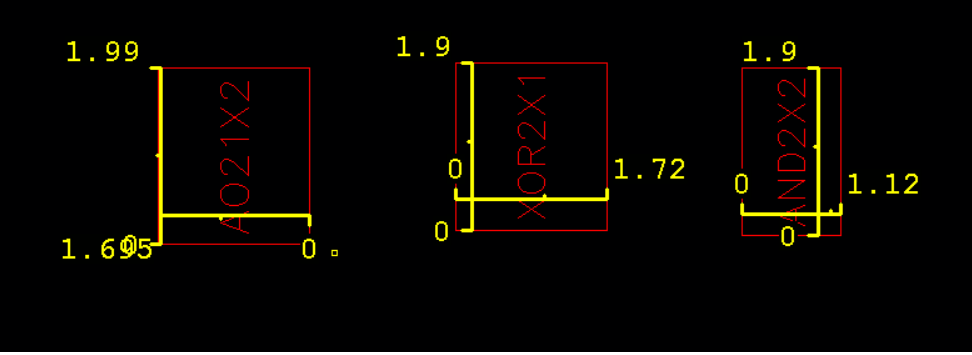
\includegraphics[width=0.7\textwidth]{images/cells_area.png}
    \caption{Cell Area Calculation}
\end{figure}

\begin{figure}[H]
    \centering
    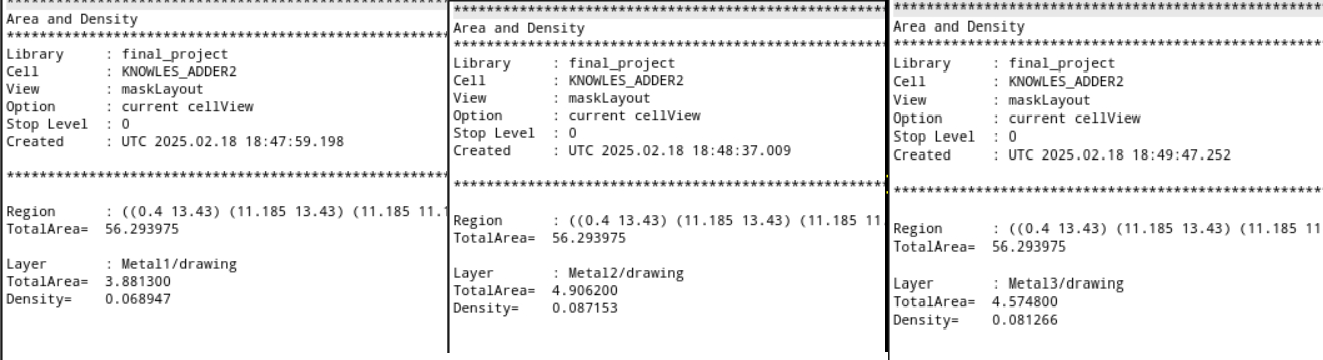
\includegraphics[width=0.7\textwidth]{images/total_area.png}
    \caption{Final Total Layout Area}
\end{figure}

\section{Verification Process}
To ensure circuit correctness, the verification was conducted in the following stages:
\begin{itemize}
    \item Initial asynchronous simulation using Logisim.
    \item Formal verification in the simulator.
    \item Manual verification using a custom script, which automated circuit validation and facilitated clock frequency testing.
\end{itemize}

Initially, I considered verifying all 4096 possible input combinations exhaustively. However, the simulator became unresponsive after approximately 100 cycles, making full verification impractical. To address this, I adopted a more feasible approach by generating random input values, ensuring a broad coverage of cases. This method, commonly used in verification processes, increased the likelihood of detecting corner cases while maintaining simulation efficiency.

\begin{figure}[H]
    \centering
    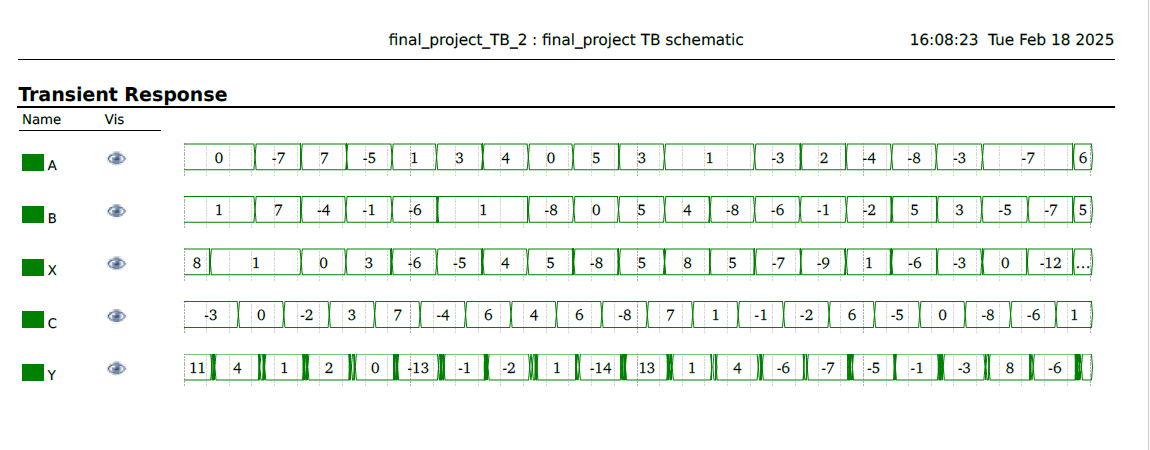
\includegraphics[width=0.8\textwidth]{graphs/wave_truth_table.png}
    \caption{Waveform truth table from the simulation.}
\end{figure}

\begin{figure}[H]
    \centering
    \begin{minipage}{0.49\textwidth}
        \centering
        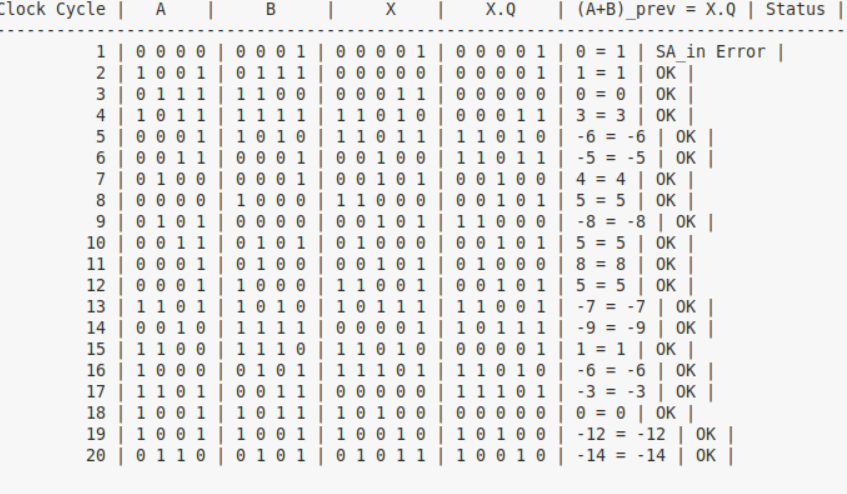
\includegraphics[width=\textwidth]{images/ADD_truth_table.png}
        \caption{Truth table verification for addition.}
    \end{minipage}
    \hfill
    \begin{minipage}{0.49\textwidth}
        \centering
        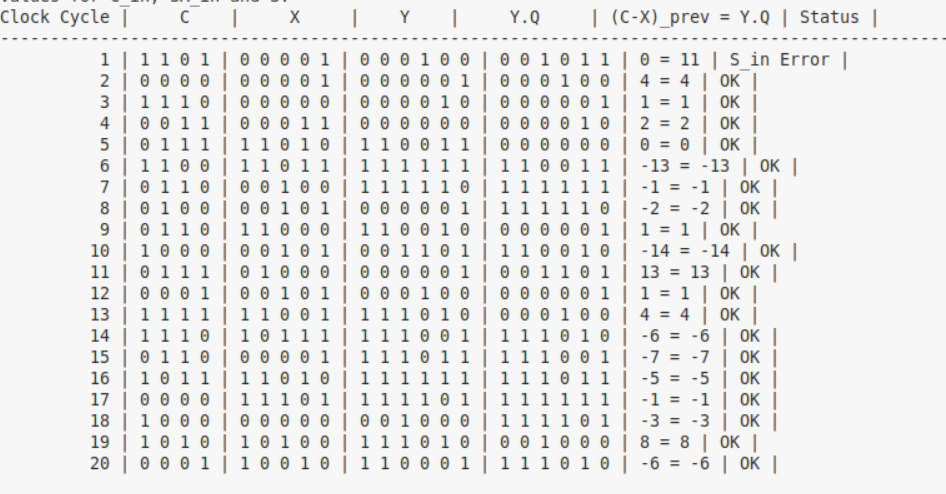
\includegraphics[width=\textwidth]{images/SUB_truth_table.png}
        \caption{Truth table verification for subtraction.}
    \end{minipage}
\end{figure}
\subsection{Design Rule Check (DRC) and Layout Versus Schematic (LVS) Validation}

To ensure the correctness of the final layout, we successfully performed both \textbf{Design Rule Check (DRC)} and \textbf{Layout Versus Schematic (LVS)} verification. The DRC confirmed that all layout rules were followed, ensuring manufacturability, while the LVS verified that the netlist extracted from the layout matched the intended schematic. 

Additionally, the extraction process was completed successfully, allowing for post-layout simulations to validate circuit performance.

\begin{figure}[H]
    \centering
    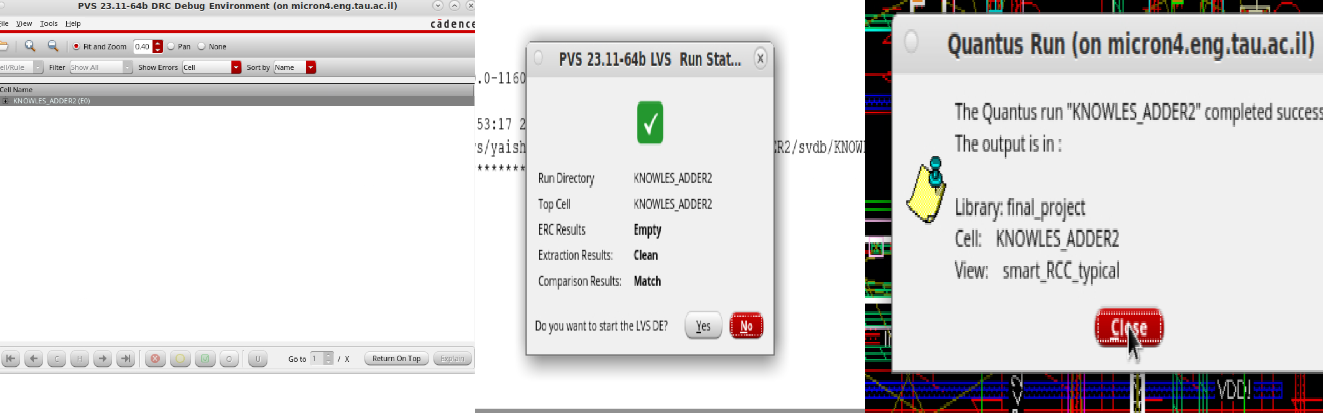
\includegraphics[width=0.7\textwidth]{images/LO_prove.png}
    \caption{Proof of successful DRC, LVS, and extraction completion}
\end{figure}




\section{ Maximum Clock Frequency}
\subsection{FF Timing Analysis}
To estimate the maximum clock frequency accurately, it was necessary to analyze the parameters of the FFs from the standard library. Unfortunately, there were no FFs with more than 4-bit width, leading to the following structure:
\begin{itemize}
    \item X was stored using a 4-bit FF and an additional single-bit FF.
    \item Y was stored using a 4-bit FF and an additional 2-bit FF.
\end{itemize}
Each component was simulated under different voltage levels to obtain reliable reference values, acknowledging that these values are non-deterministic and may vary due to multiple factors. For simplicity, it was assumed that the delay is similar across all FF outputs. Below are the extracted timing values:

\begin{table}[H]
    \centering
    \begin{tabular}{|c|c|c|c|}
        \hline
        t\textsubscript{FF} (ps) & 4-bit & 2-bit & 1-bit \\
        \hline
        Setup (1.2V/0.9V) & 13/32 & 15/36 & 21/44 \\
        \hline
        Hold (ps) & \multicolumn{3}{c|}{Around 8} \\
        \hline
        t\textsubscript{CQ} (ps) (1.2V/0.9V) & 62.2/123 & 52/104 & 45/90 \\
        \hline
    \end{tabular}
    \caption{FF Timing Characteristics with ALU as Load}
\end{table}

Key observations:
\begin{itemize}
    \item The simulations per component were crucial for accurate estimation.
    \item The drastic effect of VDD on device speed is evident.
    \item The clock-to-q (t\textsubscript{CQ}) values are significantly high and not negligible, contrary to initial expectations.
\end{itemize}

\subsection{Simulation Results}
To further analyze the timing characteristics, the following waveform comparisons were generated:

\begin{figure}[H]
    \centering
    \begin{minipage}{0.49\textwidth}
        \centering
        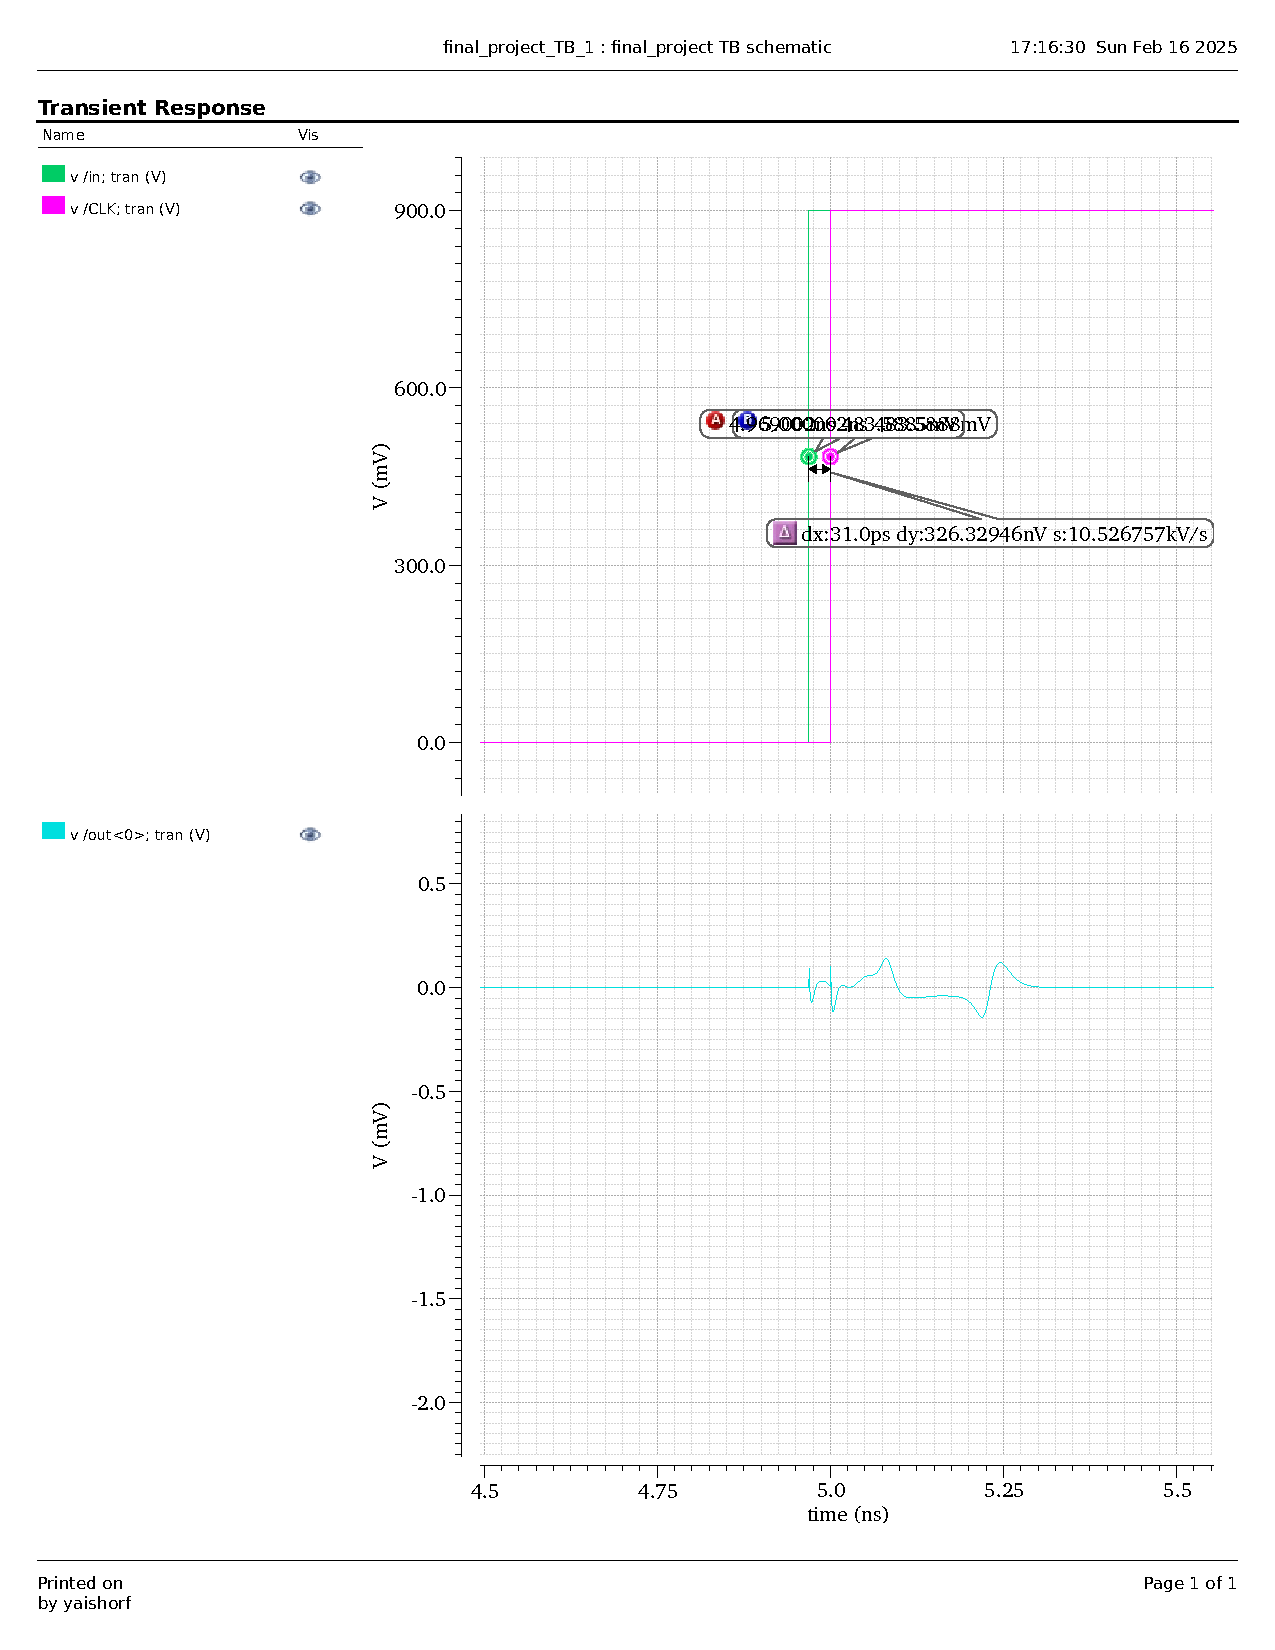
\includegraphics[width=\textwidth]{graphs/setup_0.9_31p.pdf}
        \caption{Setup time at 0.9V - 31ps.}
    \end{minipage}
    \hfill
    \begin{minipage}{0.49\textwidth}
        \centering
        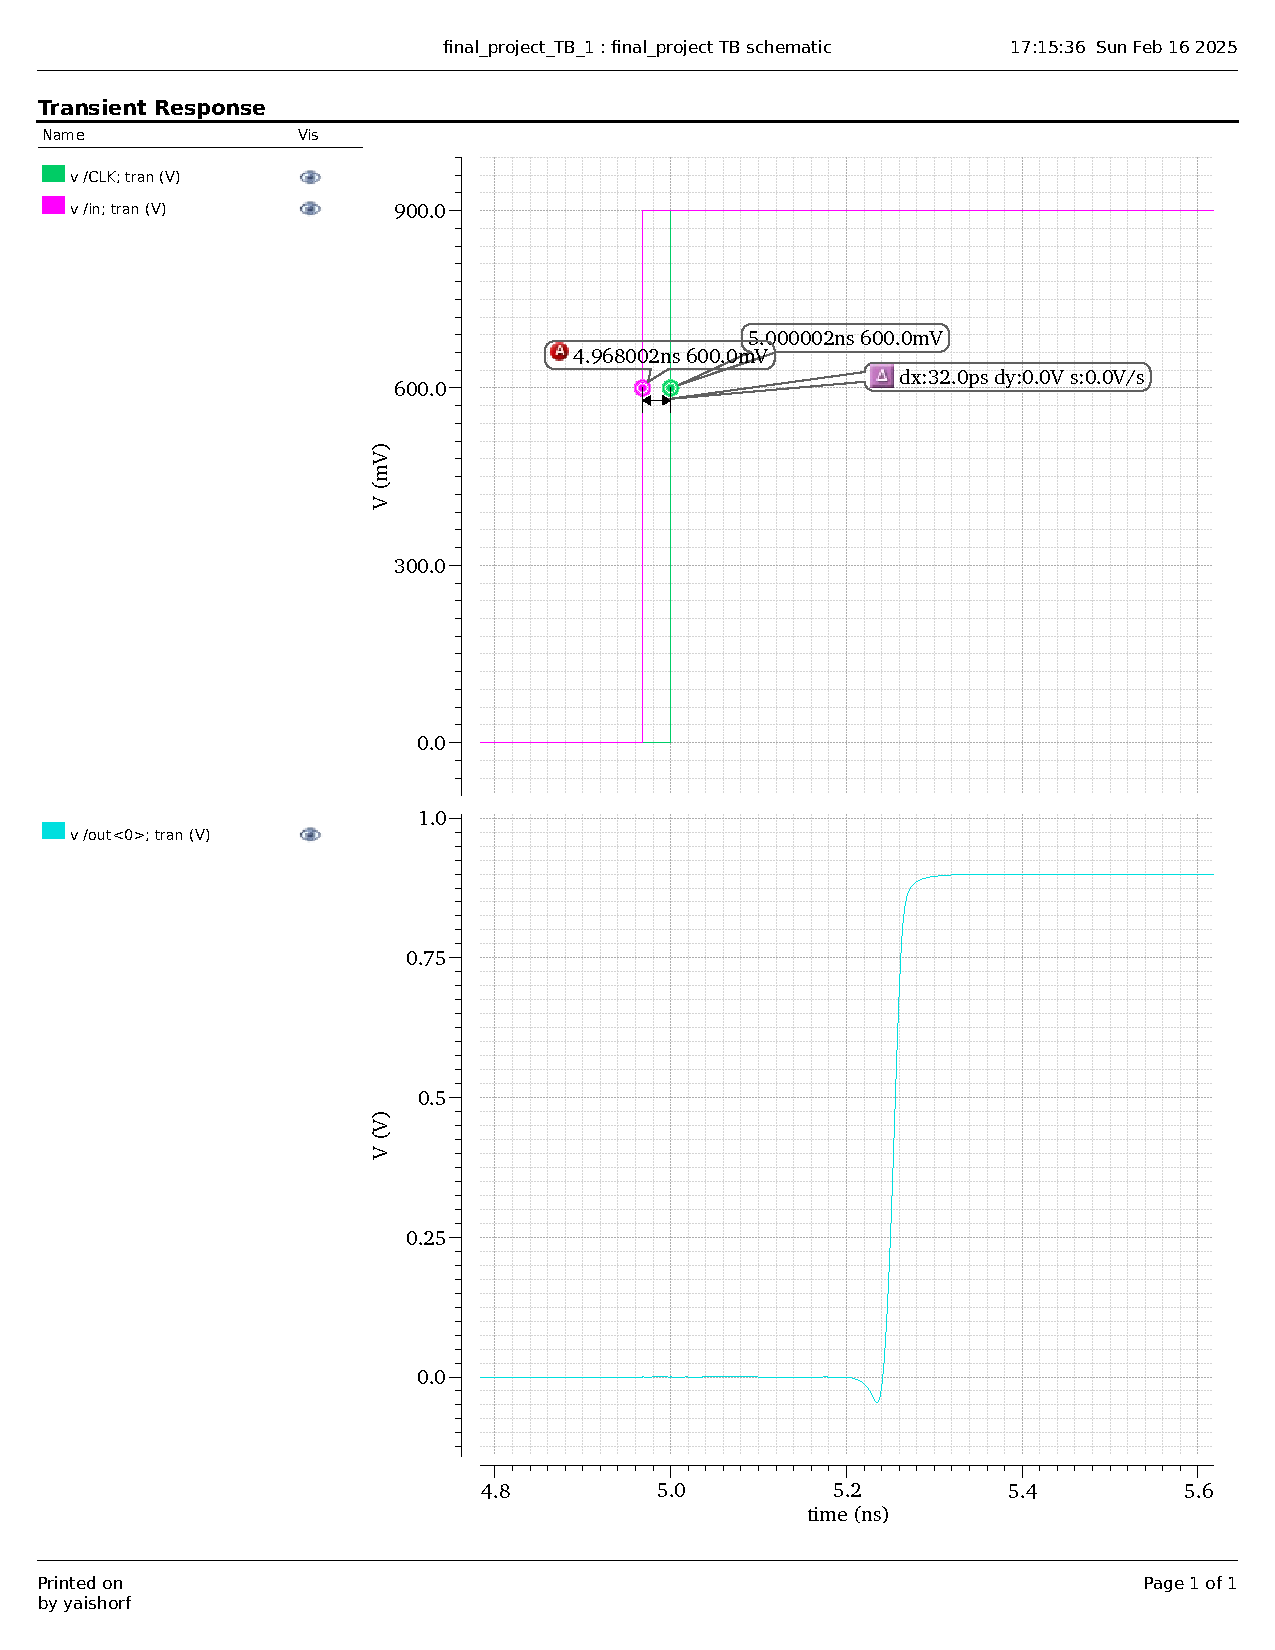
\includegraphics[width=\textwidth]{graphs/setup_0.9_32p.pdf}
        \caption{Setup time at 0.9V - 32ps.}
    \end{minipage}
\end{figure}

\begin{figure}[H]
    \centering
    \begin{minipage}{0.49\textwidth}
        \centering
        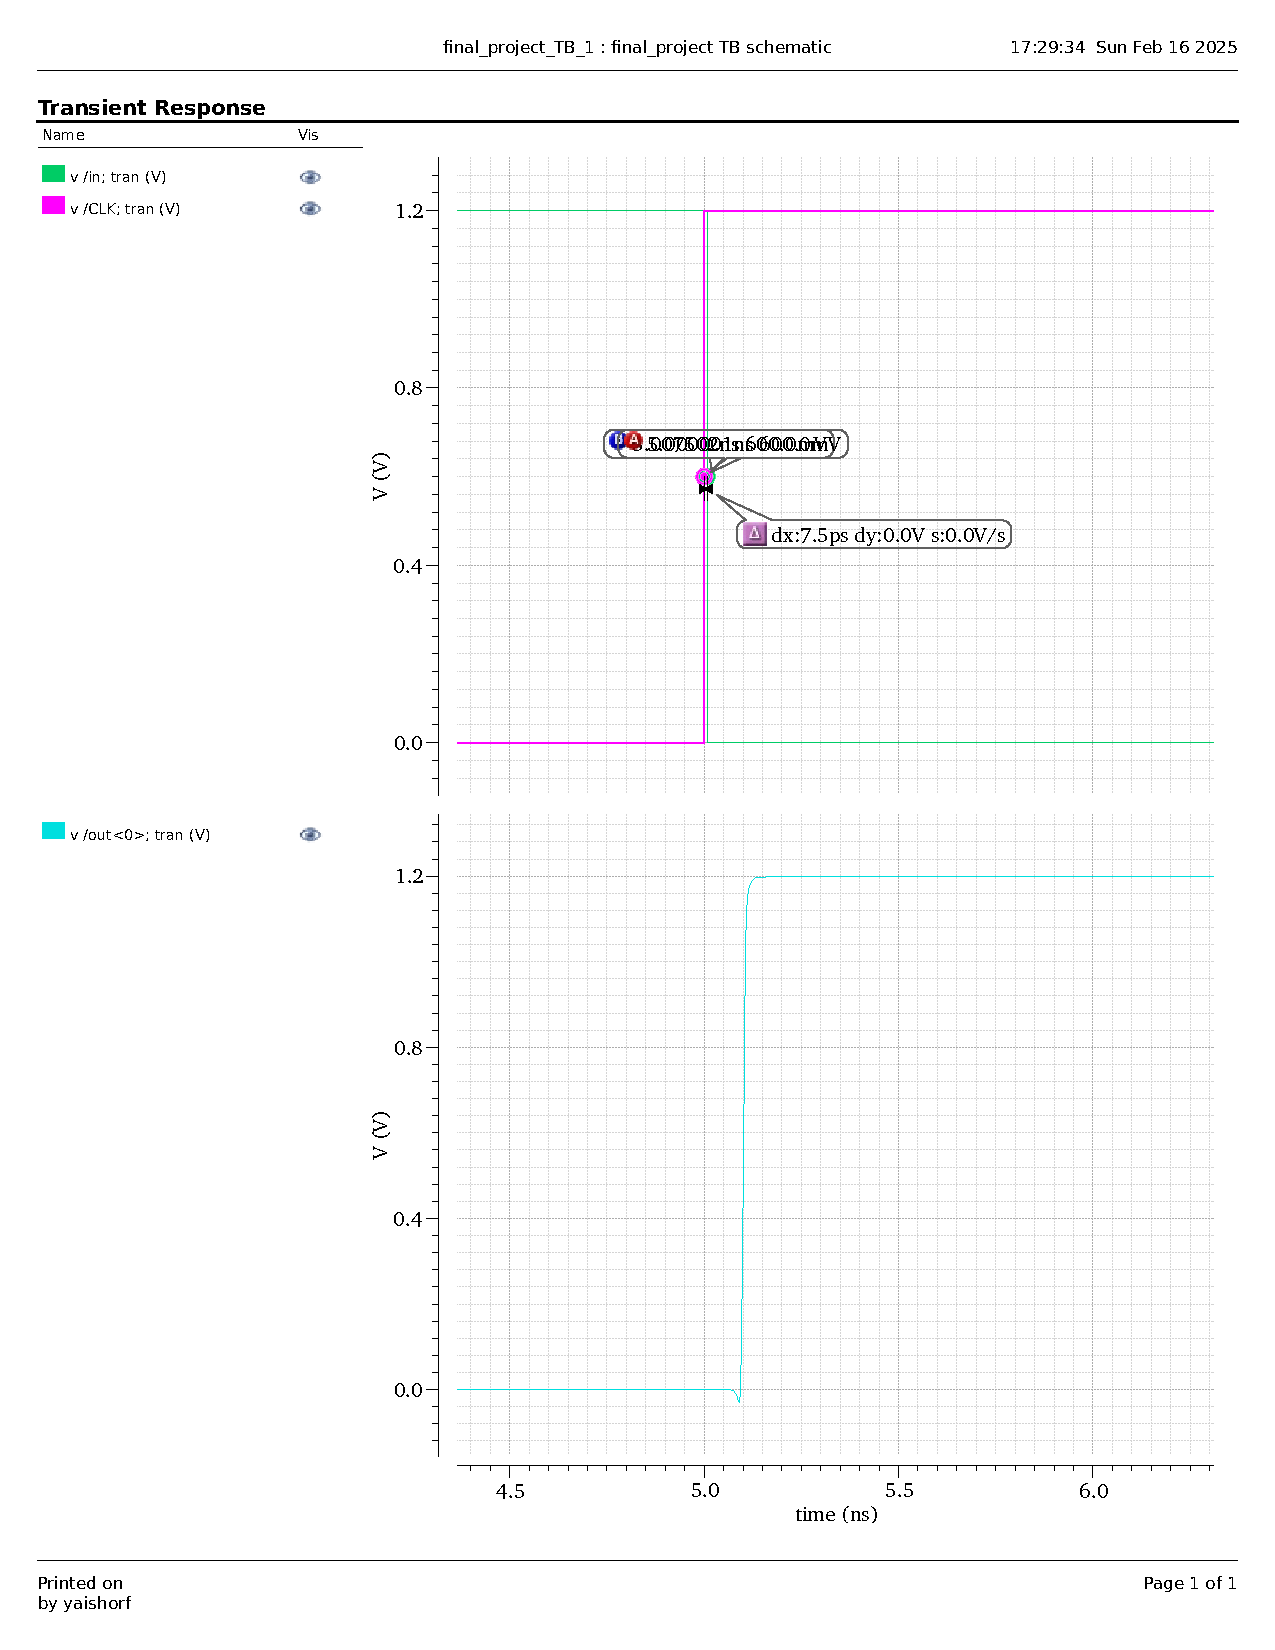
\includegraphics[width=\textwidth]{graphs/hold_1.2_7.5p.pdf}
        \caption{Hold time at 1.2V - 7.5ps.}
    \end{minipage}
    \hfill
    \begin{minipage}{0.49\textwidth}
        \centering
        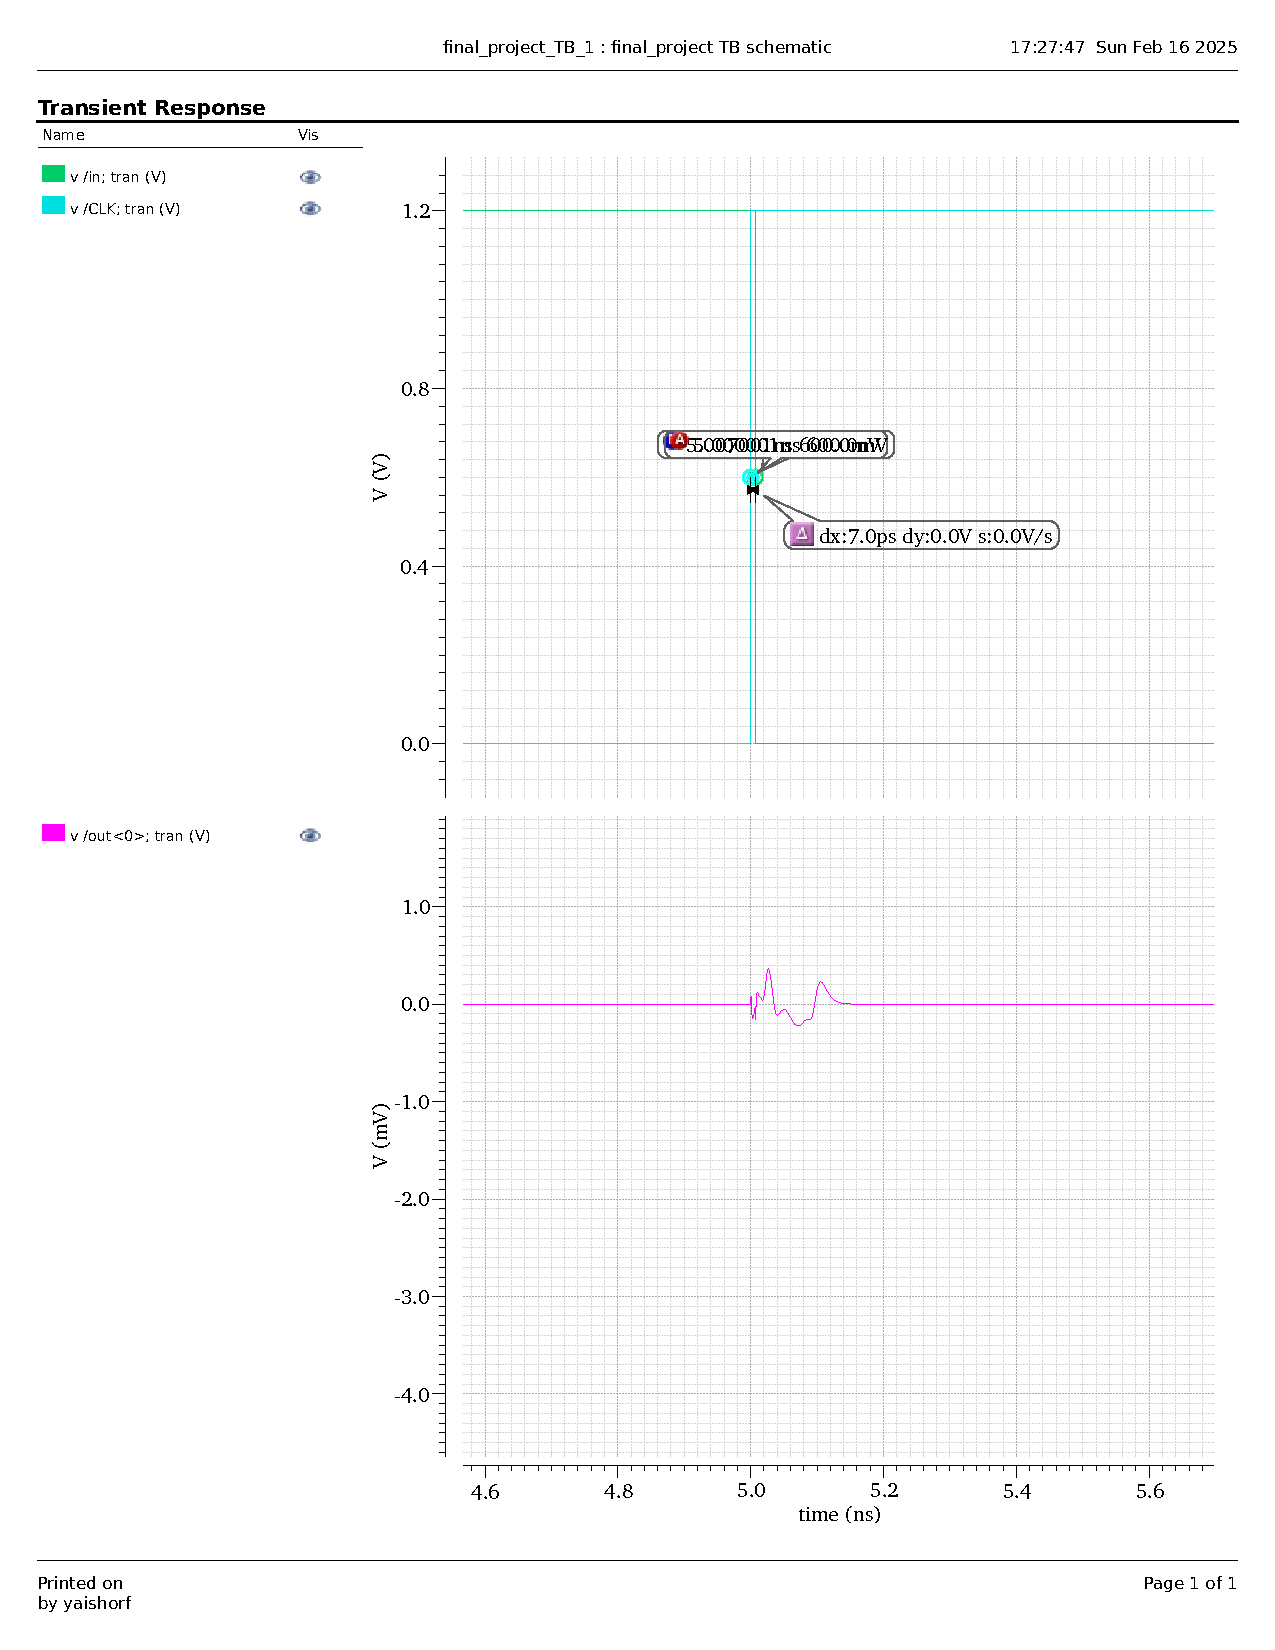
\includegraphics[width=\textwidth]{graphs/hold_1.2_7p.pdf}
        \caption{Hold time at 1.2V - 7ps.}
    \end{minipage}
\end{figure}

\begin{figure}[H]
    \centering
    \begin{minipage}{0.49\textwidth}
        \centering
        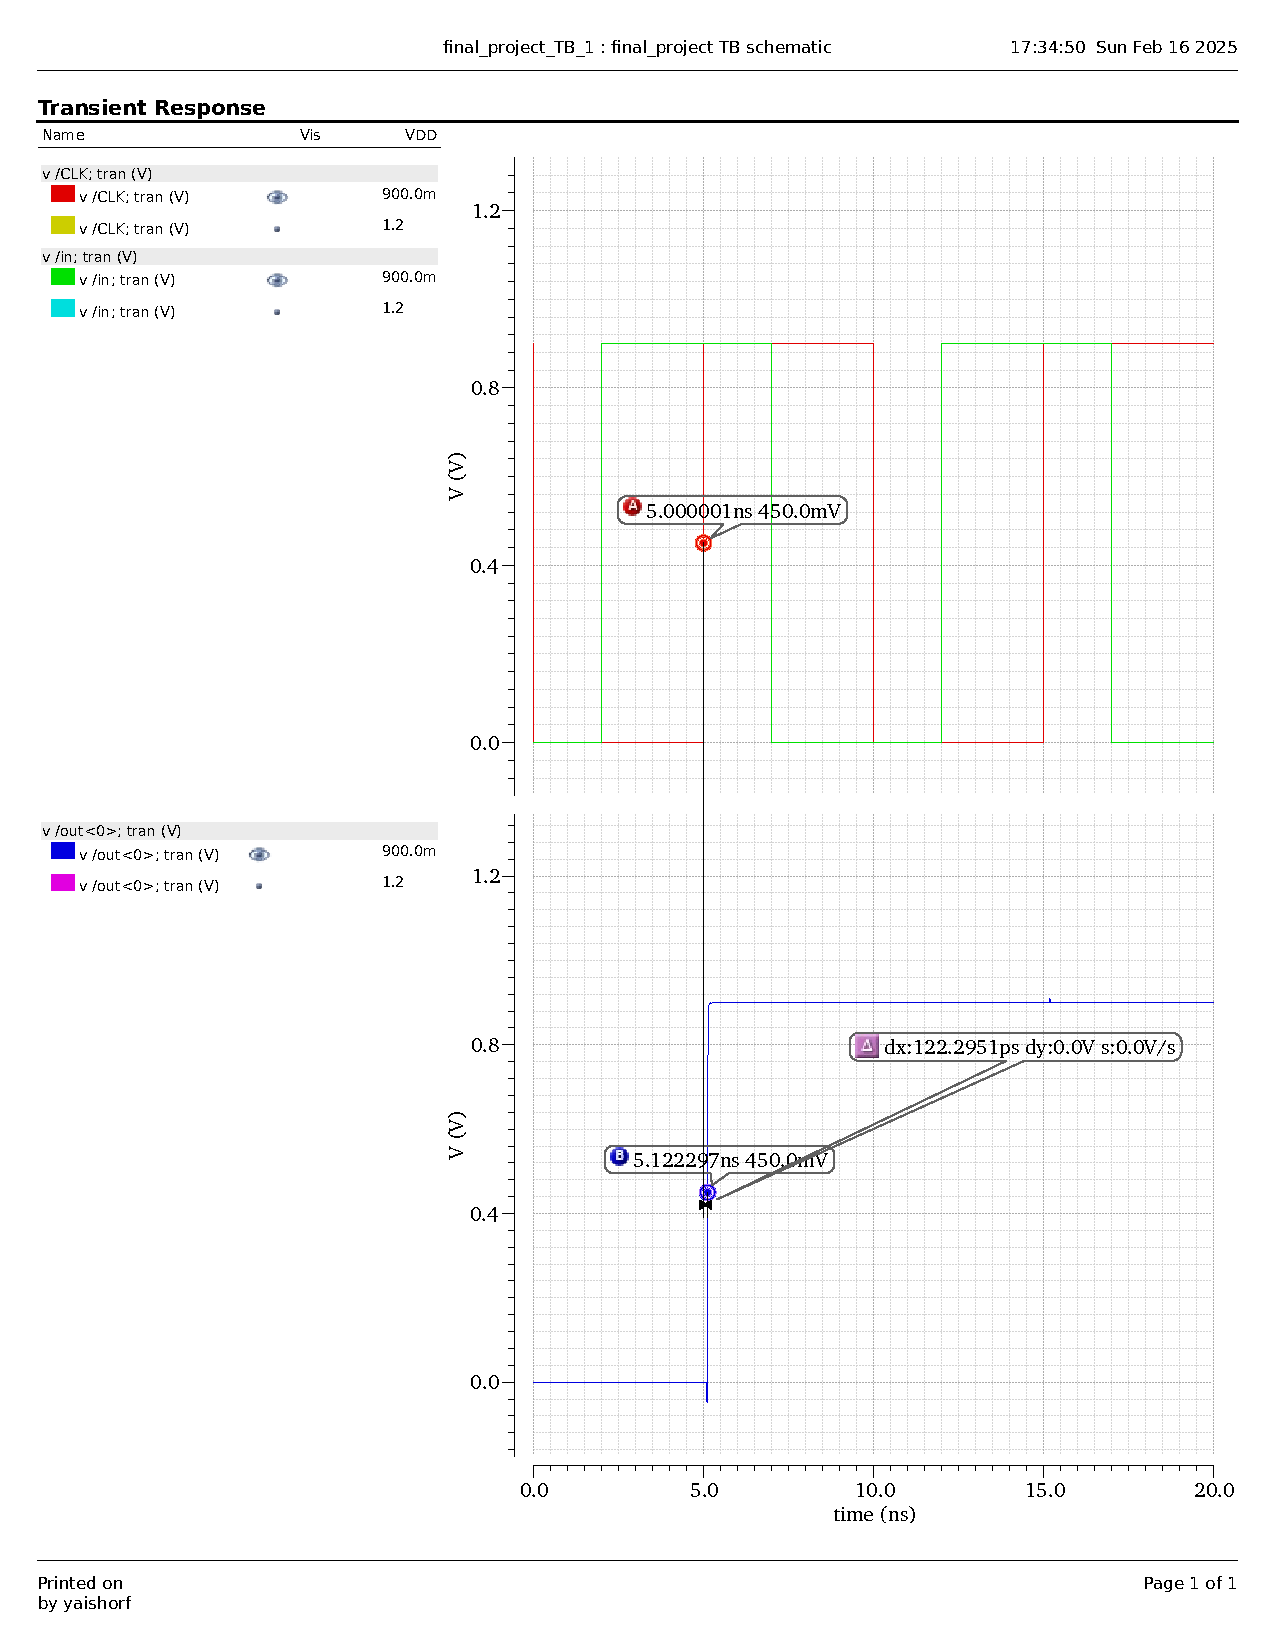
\includegraphics[width=\textwidth]{graphs/CQ_0.9_122.3p.pdf}
        \caption{Clock-to-Q delay at 0.9V - 122.3ps.}
    \end{minipage}
    \hfill
    \begin{minipage}{0.49\textwidth}
        \centering
        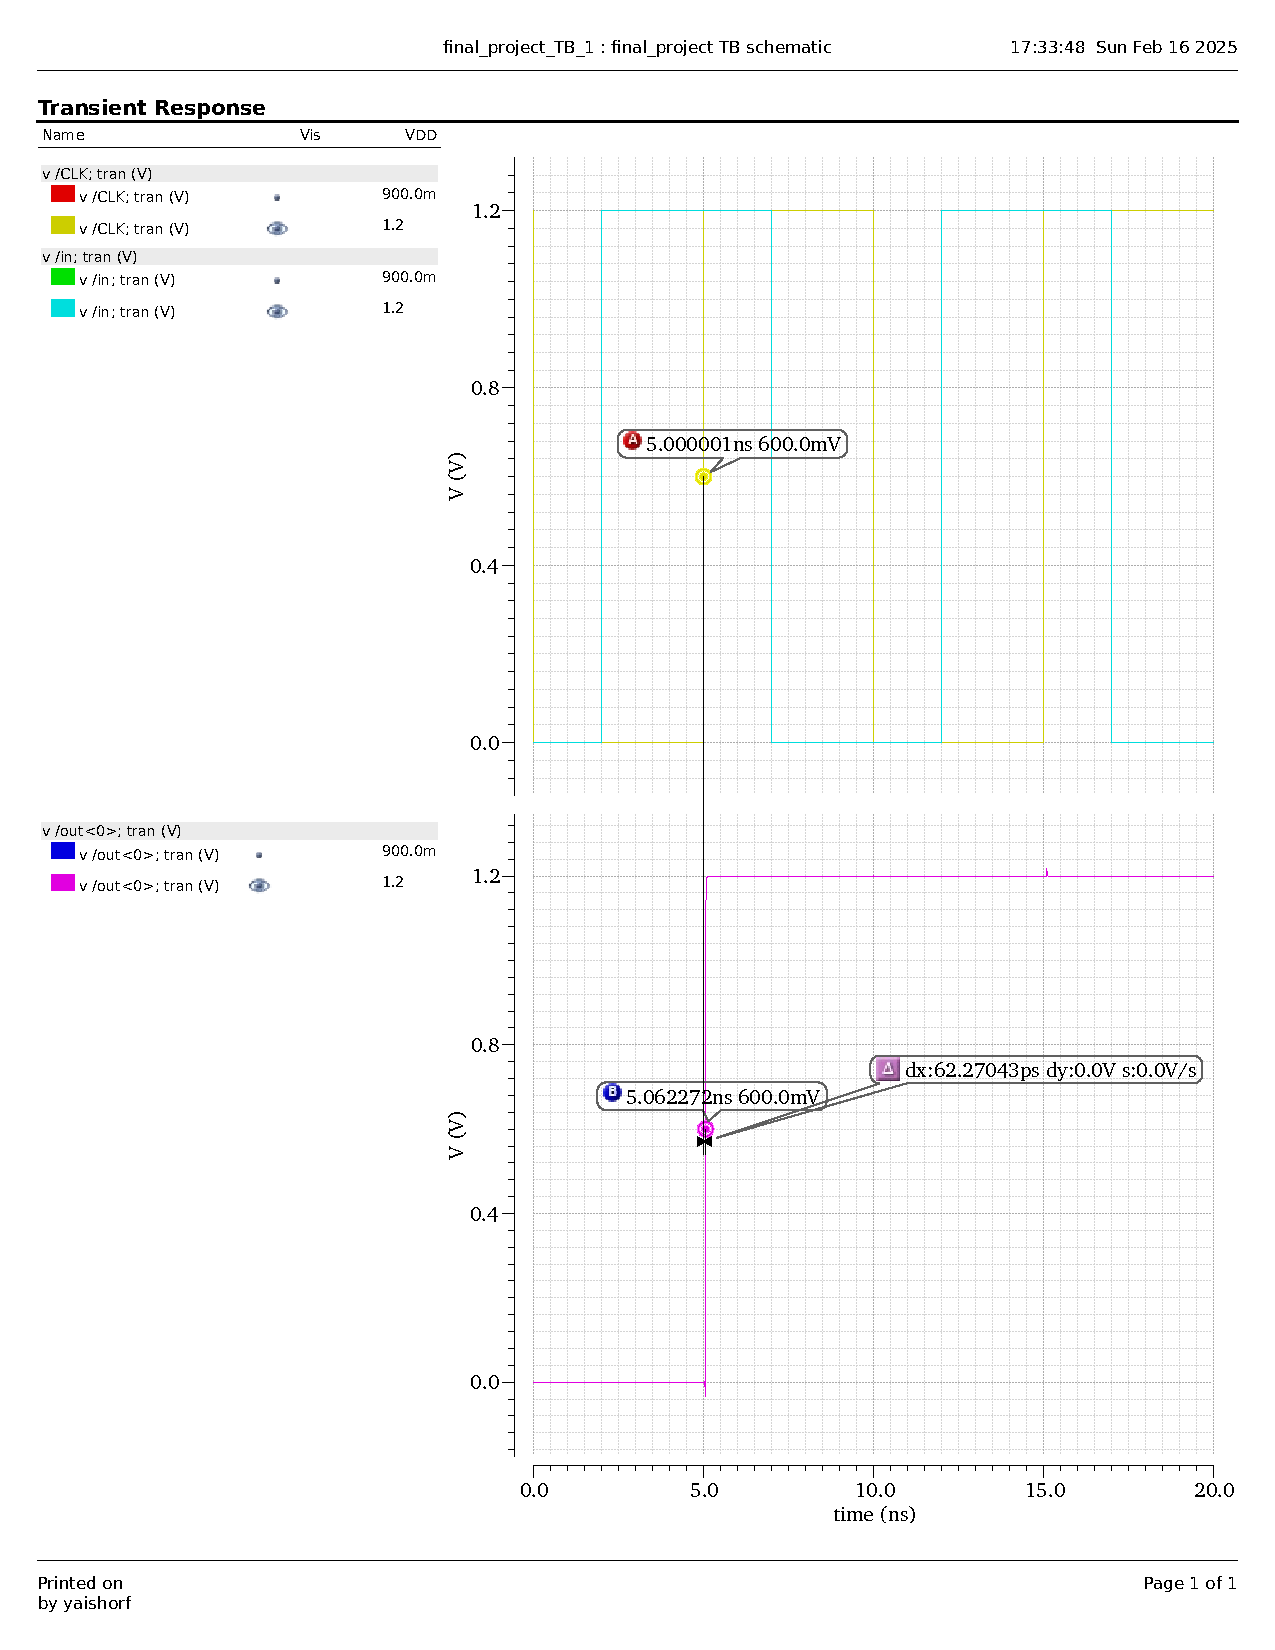
\includegraphics[width=\textwidth]{graphs/CQ_1.2_62.2p.pdf}
        \caption{Clock-to-Q delay at 1.2V - 62.2ps.}
    \end{minipage}
\end{figure}
\subsection{Finding the Critical Path}
To meet the setup and hold constraints, it was necessary to identify the critical path in both the adder and subtractor. This involved determining the minimum and maximum logical paths among all REG-to-REG paths in the different components.

Additionally, timing values for both the adder and subtractor were extracted at two supply voltages, both before and after layout extraction. Due to the complexity of analyzing these paths manually, a custom script was developed using the SKILL programming language to automate the extraction of delays for all paths. 

To ensure accuracy, FALSE PATH constraints were applied to exclude logically irrelevant connections. Specifically, input bits beyond a certain index do not impact lower-index output bits (e.g., $A[3]$ does not influence $X[0]$), and such paths were omitted from the analysis.
The following tables summarize the analysis conducted for all different scenarios:
\begin{table}[h]
\caption{Delays for the ADDER}
\begin{tabular}{||c|c|c|c||}
\hline
\textbf{Start Point} & \textbf{End Point} & \textbf{Before Extraction (0.9V/1.2V)} & \textbf{After Extraction (0.9V/1.2V)} \\
\hline\hline
A\_in<0> & SA<0> & 87.0/43.0 & 157.8/75.4 \\
\hline
A\_in<0> & SA<1> & 122.3/58.9 & 254.2/121.5 \\
\hline
B\_in<0> & SA<1> & 138.3/67.6 & 281.2/130.9 \\
\hline
A\_in<1> & SA<1> & 167.9/84.3 & 279.2/138.0 \\
\hline
B\_in<1> & SA<1> & 121.3/57.5 & 253.1/125.9 \\
\hline
A\_in<0> & SA<2> & 133.2/63.6 & 259.2/126.1 \\
\hline
B\_in<1> & SA<2> & 131.2/62.2 & 254.8/123.4 \\
\hline
B\_in<2> & SA<2> & 131.2/62.2 & 254.1/123.0 \\
\hline
A\_in<0> & SA<3> & 140.2/66.9 & 271.8/132.2 \\
\hline
B\_in<1> & SA<3> & 147.3/70.5 & 292.8/140.3 \\
\hline
B\_in<2> & SA<3> & 138.2/65.5 & 266.7/129.1 \\
\hline
A\_in<3> & SA<3> & 156.0/75.6 & 303.2/146.3 \\
\hline
A\_in<0> & SA<4> & 152.3/73.0 & 297.4/145.0 \\
\hline
B\_in<0> & SA<4> & 191.6/90.4 & 382.6/181.4 \\
\hline
B\_in<1> & SA<4> & 157.3/76.4 & 325.7/156.7 \\
\hline
A\_in<2> & SA<4> & 218.1/101.6 & 465.3/219.2 \\
\hline
B\_in<2> & SA<4> & 150.3/71.6 & 292.3/141.9 \\
\hline
A\_in<3> & SA<4> & 169.8/82.5 & 334.3/162.0 \\
\hline
B\_in<0> & SA<2> & -/- & 406.4/197.4 \\
\hline
A\_in<1> & SA<2> & -/- & 384.8/183.0 \\
\hline
A\_in<2> & SA<2> & -/- & 332.7/160.5 \\
\hline
B\_in<0> & SA<3> & -/- & 268.9/128.6 \\
\hline
\end{tabular}
\end{table}

\begin{table}[H]
\caption{Delays for the SUBSTRACTOR}
\begin{tabular}{||c|c|c|c||}
\hline
\textbf{Start Point} & \textbf{End Point} & \textbf{0.9V (pS)} & \textbf{1.2V (pS)} \\
\hline\hline
C\_in<0> & S<0> & 110.5 & - \\
\hline
SA\_in<0> & S<0> & 82.8 & 39.3 \\
\hline
C\_in<0> & S<1> & 125.7 & - \\
\hline
SA\_in<0> & S<1> & 162.2 & 80.1 \\
\hline
C\_in<1> & S<1> & 145.7 & - \\
\hline
C\_in<0> & S<2> & 151.9 & - \\
\hline
C\_in<2> & S<2> & 145.9 & - \\
\hline
SA\_in<0> & S<2> & - & 114.2 \\
\hline
C\_in<0> & S<3> & 145.3 & - \\
\hline
C\_in<2> & S<3> & 145.2 & - \\
\hline
C\_in<3> & S<3> & 141.7 & - \\
\hline
SA\_in<0> & S<3> & - & 73.8 \\
\hline
SA\_in<3> & S<3> & - & 57.8 \\
\hline
C\_in<0> & S<4> & 146.1 & 70.4 \\
\hline
C\_in<2> & S<4> & 146.0 & 70.4 \\
\hline
C\_in<3> & S<4> & 142.5 & 68.0 \\
\hline
C\_in<0> & S<5> & 158.2 & 76.5 \\
\hline
C\_in<2> & S<5> & 158.2 & 76.5 \\
\hline
C\_in<3> & S<5> & 154.6 & 74.1 \\
\hline
\end{tabular}
\end{table}




\begin{table}[H]
\caption{Maximum and Minimum Delays Summary}
\resizebox{\textwidth}{!}{
\begin{tabular}{||c|c|c|c|c|c|c||}
\hline
\textbf{Component} & \textbf{Condition} & \textbf{Voltage} & \textbf{Min Delay (pS)} & \textbf{Max Delay (pS)} & \textbf{Min Path} & \textbf{Max Path} \\
\hline\hline
\multirow{4}{*}{ADDER} & \multirow{2}{*}{Before EX} & 0.9V & 87.0 & 336.9 & A\_in<0> → SA<0> & B\_in<0> → SA<4> \\
& & 1.2V & 43.0 & 150.8 & A\_in<0> → SA<0> & B\_in<0> → SA<4> \\
\cline{2-7}
& \multirow{2}{*}{After EX} & 0.9V & 157.8 & 598.8 & A\_in<0> → SA<0> & B\_in<0> → SA<4> \\
& & 1.2V & 75.4 & 279.4 & A\_in<0> → SA<0> & B\_in<0> → SA<4> \\
\hline
\multirow{2}{*}{SUBSTRACTOR} & \multirow{2}{*}{-} & 0.9V & 82.8 & 162.2 & SA\_in<0> → S<0> & SA\_in<0> → S<1> \\
& & 1.2V & 39.3 & 114.2 & SA\_in<0> → S<0> & SA\_in<0> → S<2> \\
\hline
\end{tabular}
}
\end{table}
\begin{enumerate}
    \item \textbf{Extraction Impact:}
        \begin{itemize}
            \item The delays after extraction are approximately doubled compared to before extraction in the ADDER
            \item The critical path (B\_in<0> → SA<4>) remains consistent before and after extraction
        \end{itemize}
    
    \item \textbf{Voltage Impact:}
        \begin{itemize}
            \item At 1.2V, delays are consistently shorter than at 0.9V by approximately 50\%
            \item This voltage effect is observed in both ADDER and SUBSTRACTOR
        \end{itemize}
    
    \item \textbf{Component Analysis:}
        \begin{itemize}
            \item ADDER delays after extraction are significantly larger due to the extraction process
            \item SUBSTRACTOR delays cannot be directly compared with ADDER as it hasn't undergone extraction
            \item A fair comparison would require extraction data for both components
        \end{itemize}
    
    \item \textbf{Critical Paths:}
        \begin{itemize}
            \item ADDER maintains the same critical paths (both min and max) across all conditions
            \item SUBSTRACTOR shows different maximum critical paths at different voltages, while maintaining the same minimum critical path
        \end{itemize}

    \item \textbf{Expected vs. Actual Results:}
        \begin{itemize}
            \item Most paths behaved as expected, with longer paths showing maximum delays and shorter paths showing minimum delays
            \item However, some paths exhibited higher delays than anticipated based on their path length
            \item This suggests that factors beyond path length, such as load capacitance and gate complexity, significantly influence the delay
        \end{itemize}
\end{enumerate}
\subsubsection{Critical Path Delay Verification}

To further validate the critical path delays, timing analysis was conducted using waveform diagrams. The analysis includes both the \textbf{minimum delay path} and the \textbf{maximum delay path} for both the adder and subtractor circuits. The verification was performed at two supply voltages (1.2V and 0.9V) before and after extraction.

The following figures illustrate the measured signal delays:

\begin{figure}[H]
    \centering
    \begin{minipage}{0.49\textwidth}
        \centering
        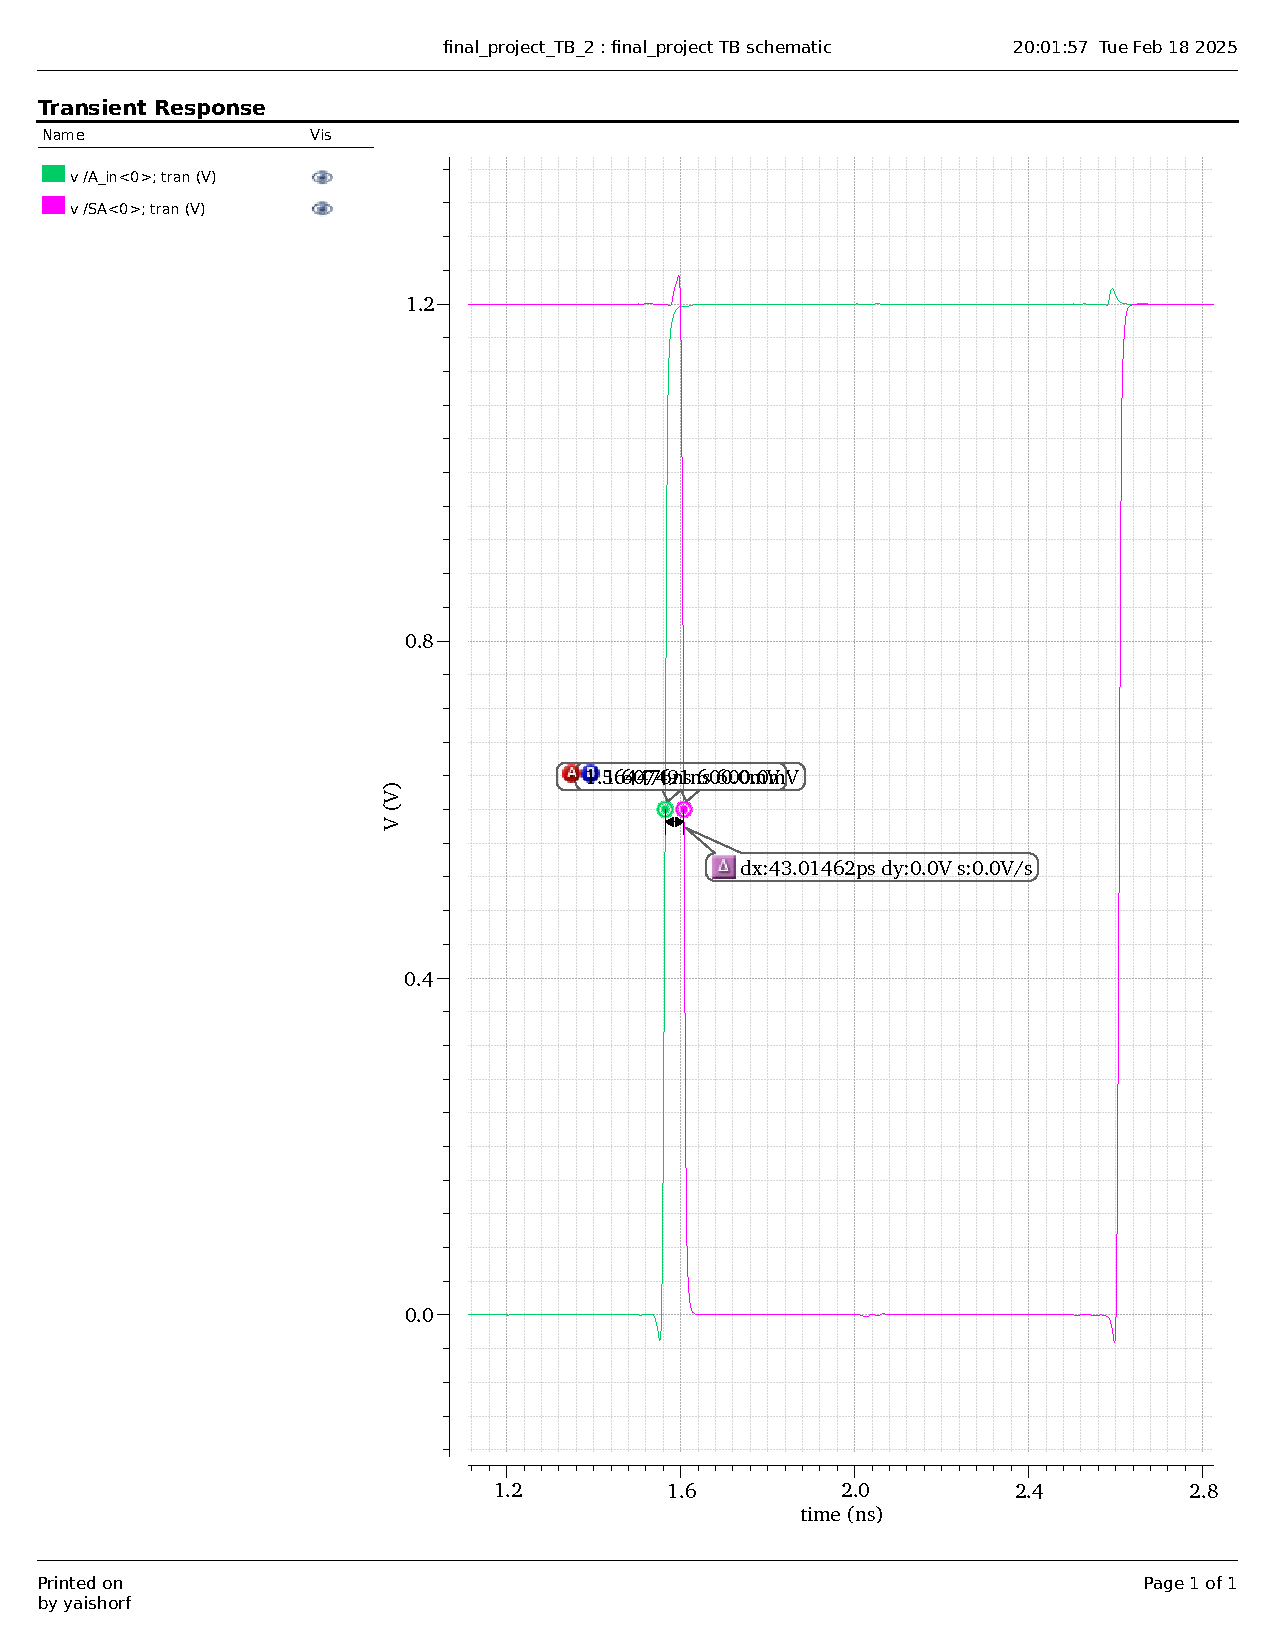
\includegraphics[width=\textwidth]{delay/CP_min_add_1.2.pdf}
        \caption{Minimum delay path - Adder @ 1.2V}
    \end{minipage}
    \hfill
    \begin{minipage}{0.49\textwidth}
        \centering
        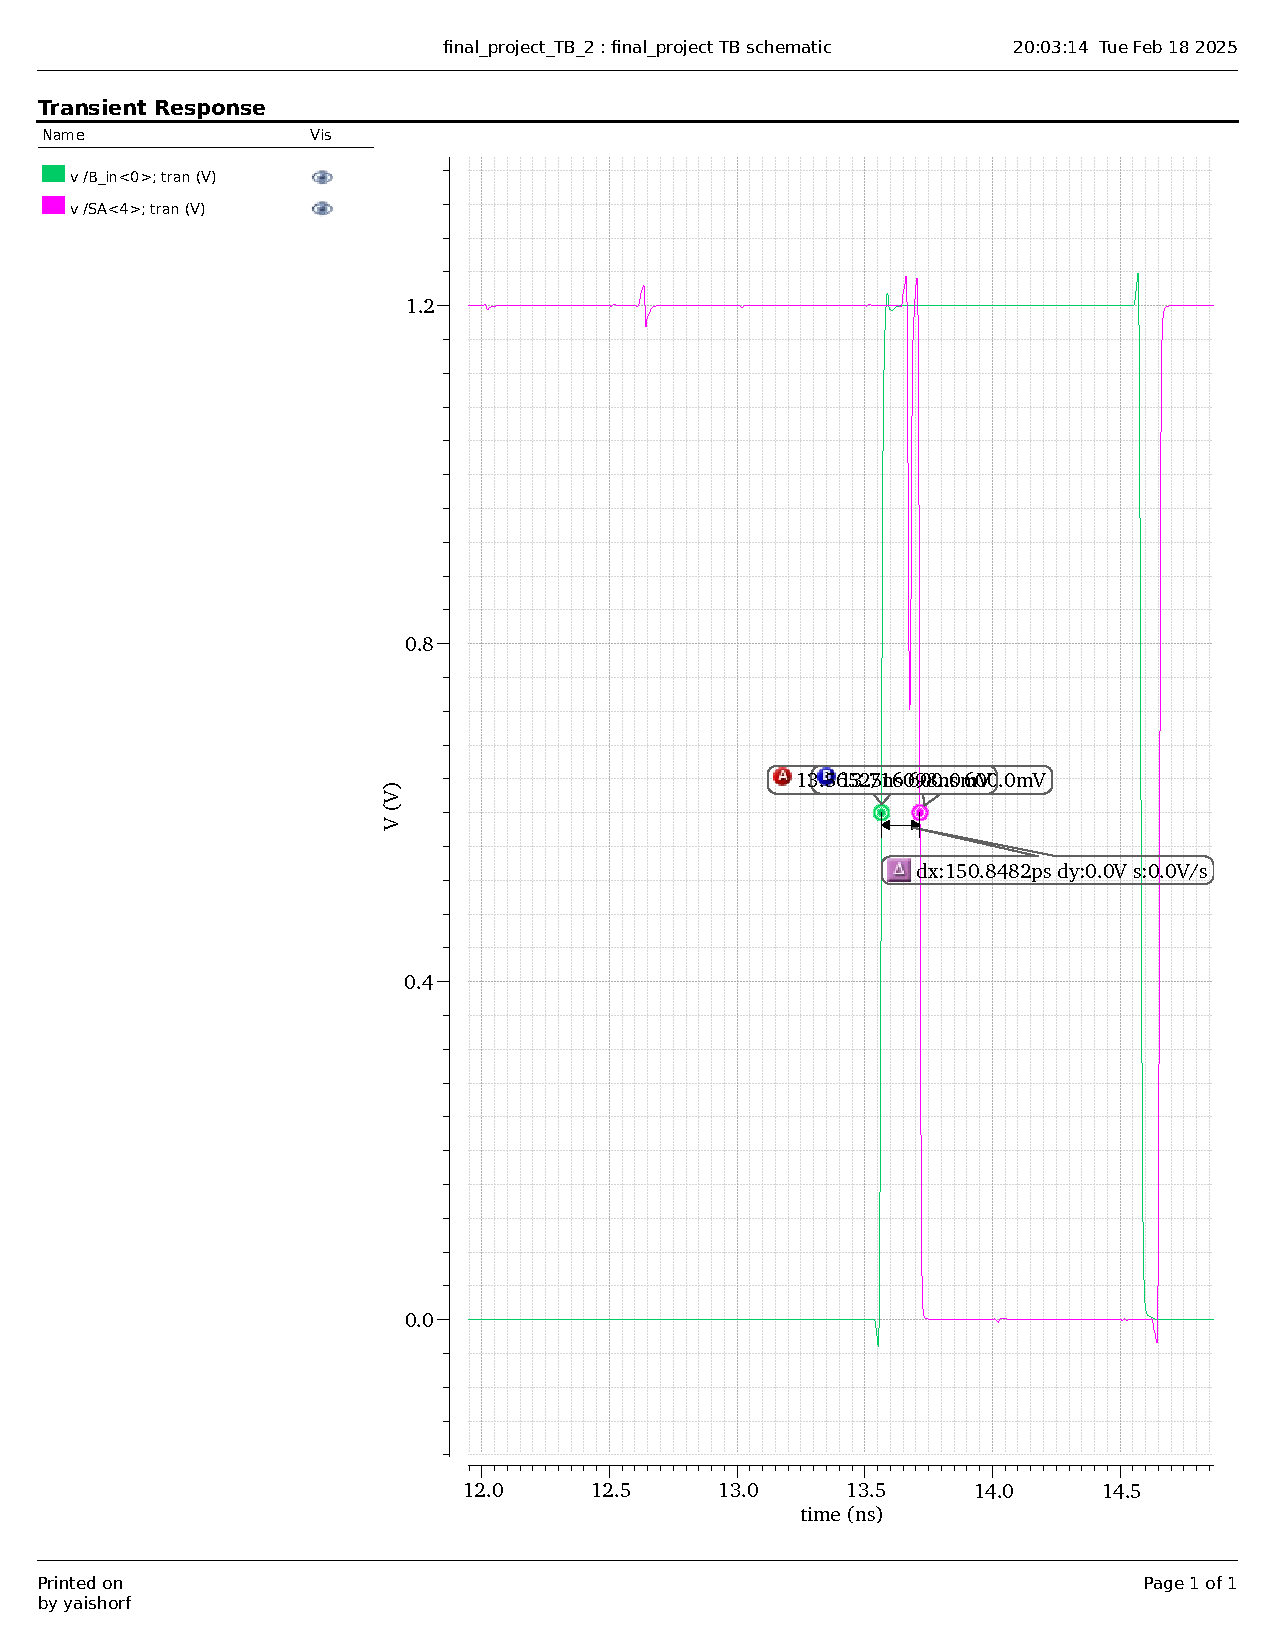
\includegraphics[width=\textwidth]{delay/CP_max1_add_1.2.pdf}
        \caption{Maximum delay path - Adder @ 1.2V}
    \end{minipage}
\end{figure}

\begin{figure}[H]
    \centering
    \begin{minipage}{0.49\textwidth}
        \centering
        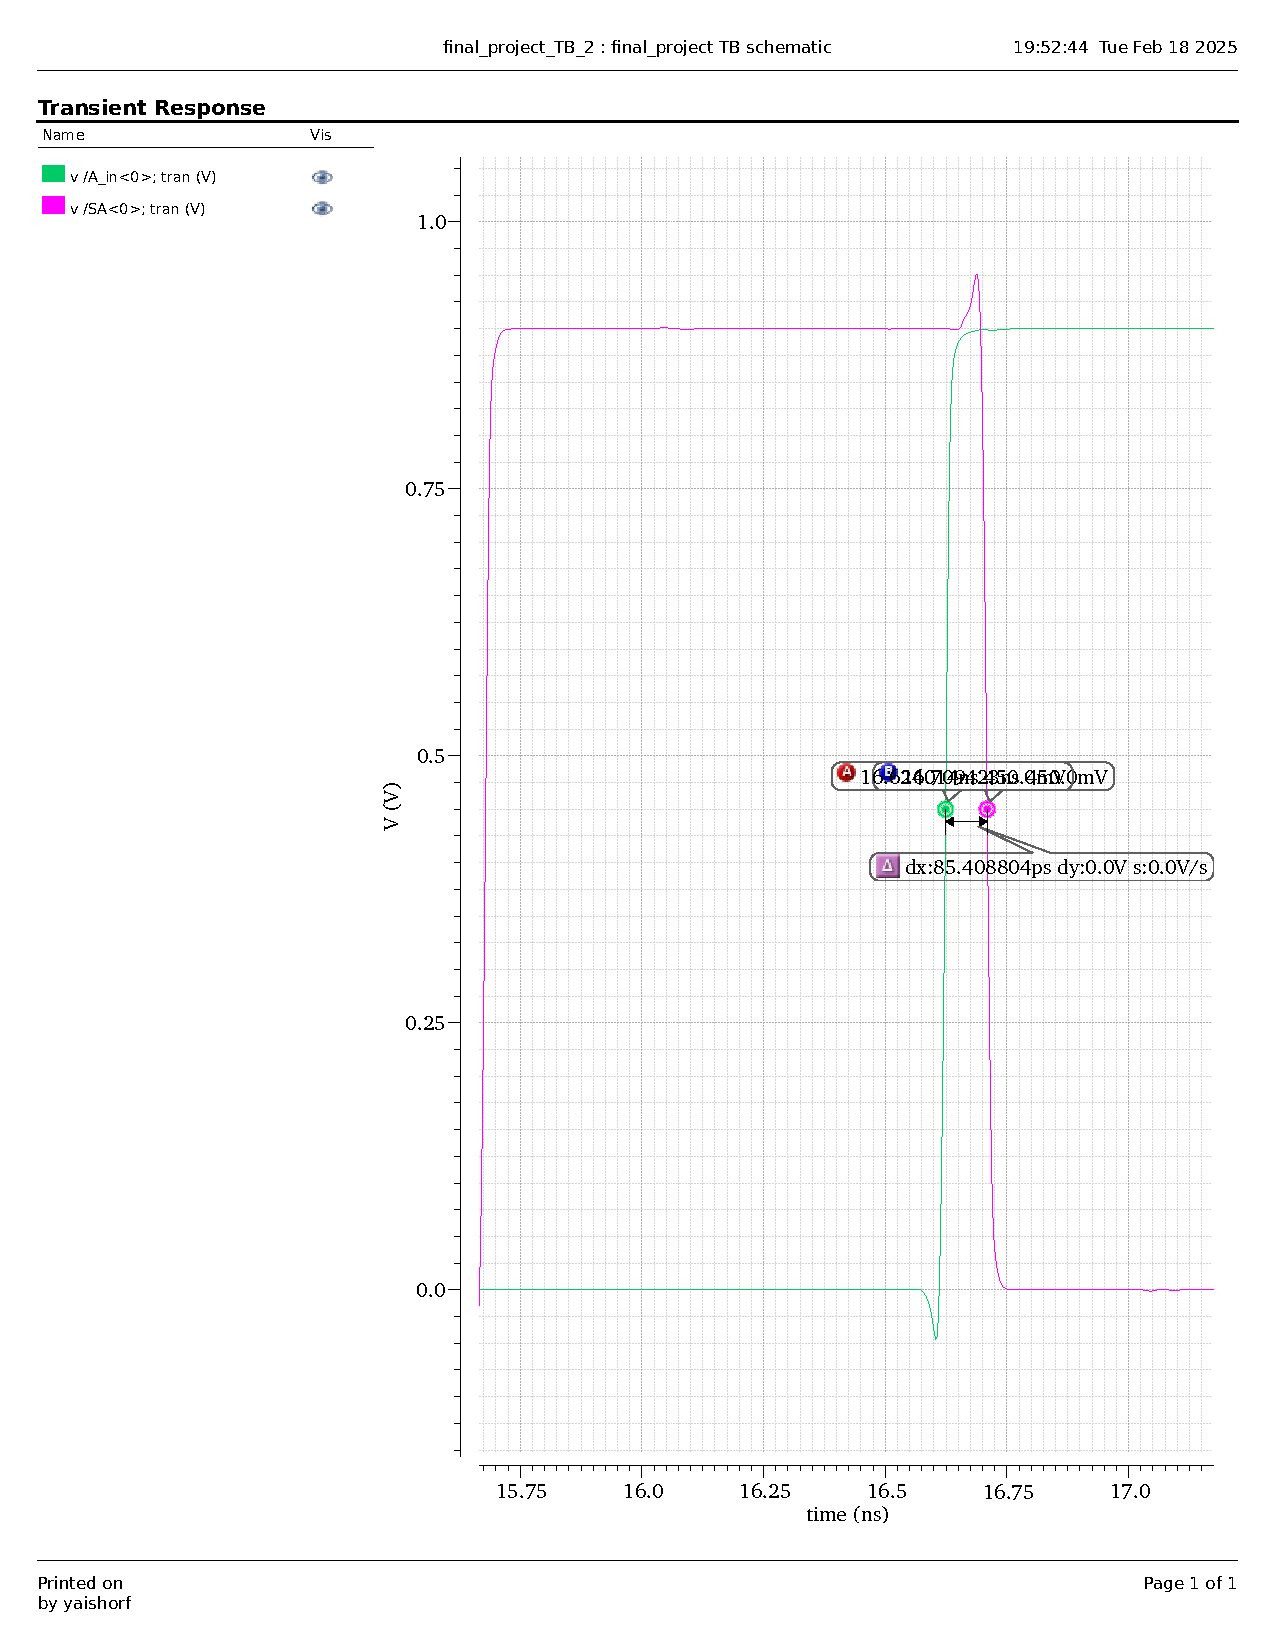
\includegraphics[width=\textwidth]{delay/CP_min_add_0.9.pdf}
        \caption{Minimum delay path - Adder @ 0.9V}
    \end{minipage}
    \hfill
    \begin{minipage}{0.49\textwidth}
        \centering
        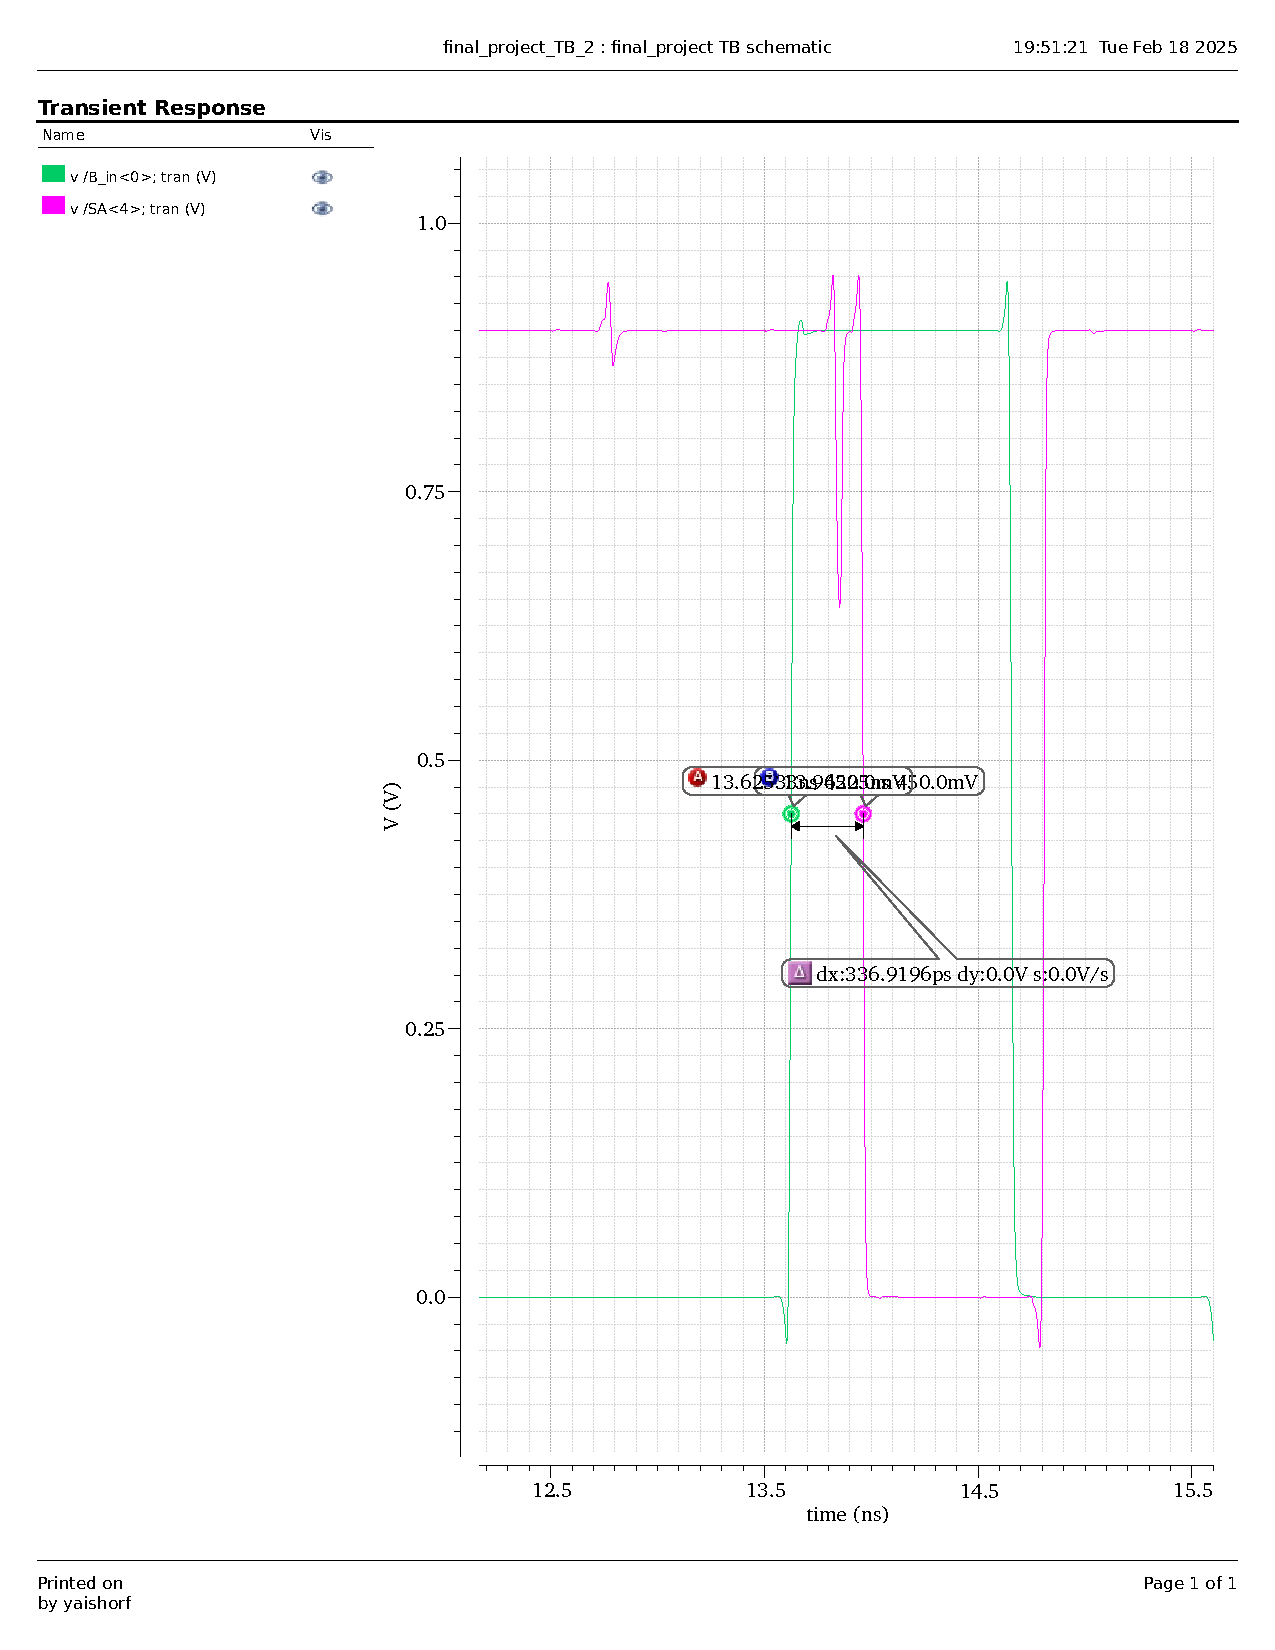
\includegraphics[width=\textwidth]{delay/CP_max_add_0.9.pdf}
        \caption{Maximum delay path - Adder @ 0.9V}
    \end{minipage}
\end{figure}

\begin{figure}[H]
    \centering
    \begin{minipage}{0.49\textwidth}
        \centering
        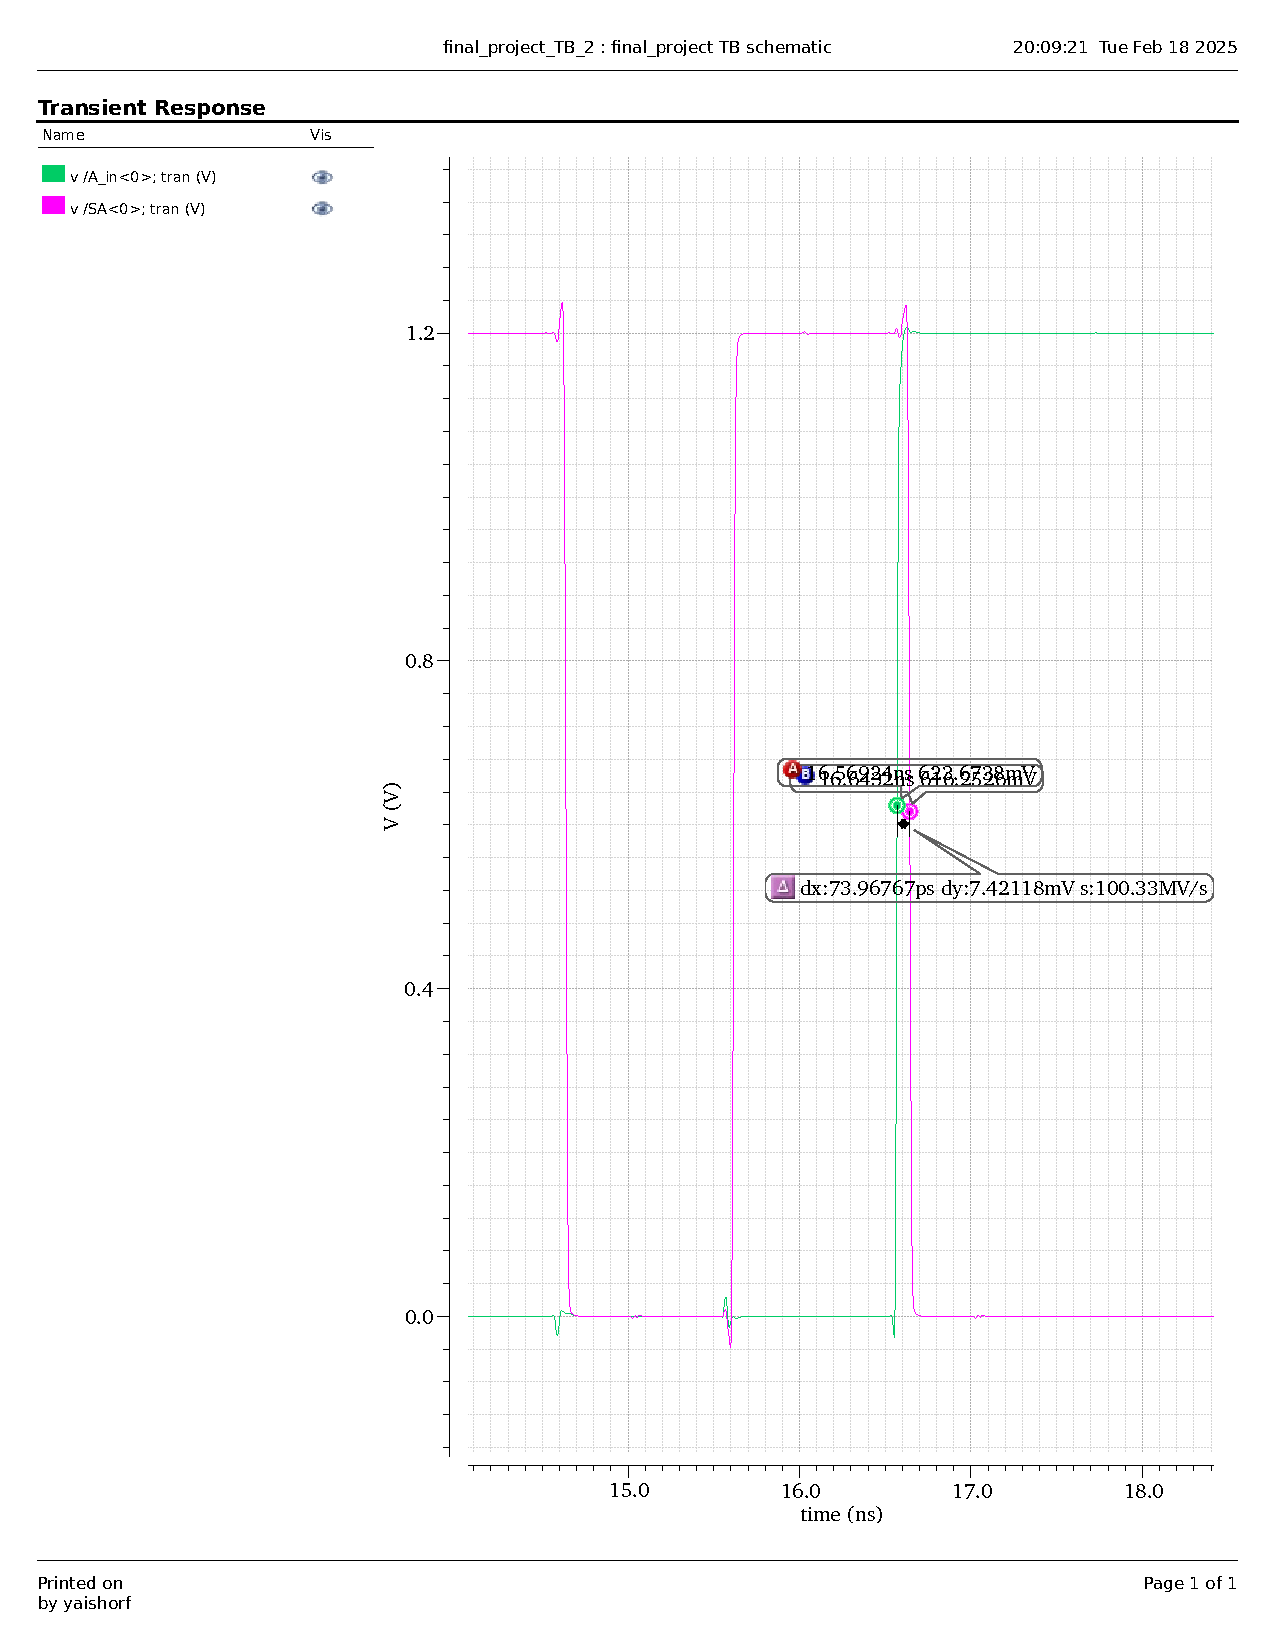
\includegraphics[width=\textwidth]{delay/CP_min_add_1.2_ex.pdf}
        \caption{Minimum delay path - Adder @ 1.2V (After Extraction)}
    \end{minipage}
    \hfill
    \begin{minipage}{0.49\textwidth}
        \centering
        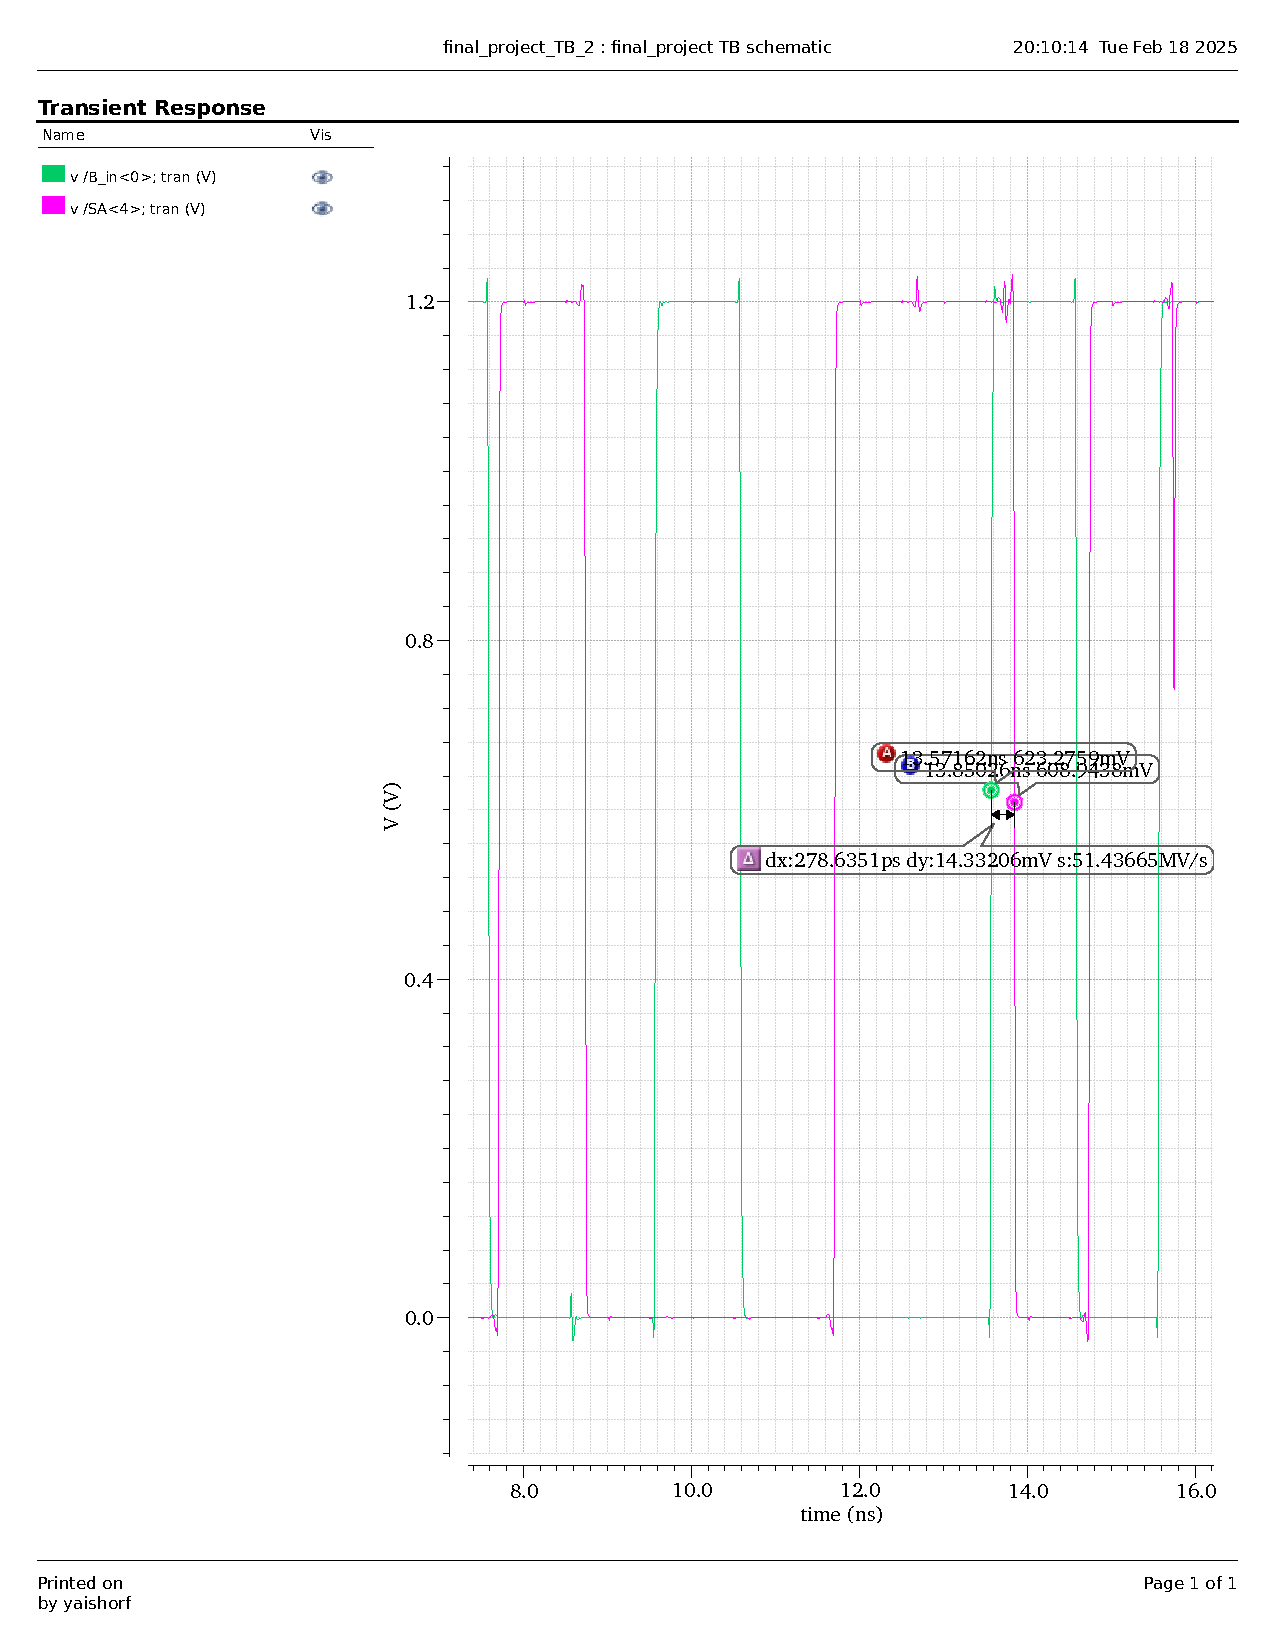
\includegraphics[width=\textwidth]{delay/CP_max_add_1.2_ex.pdf}
        \caption{Maximum delay path - Adder @ 1.2V (After Extraction)}
    \end{minipage}
\end{figure}

\begin{figure}[H]
    \centering
    \begin{minipage}{0.49\textwidth}
        \centering
        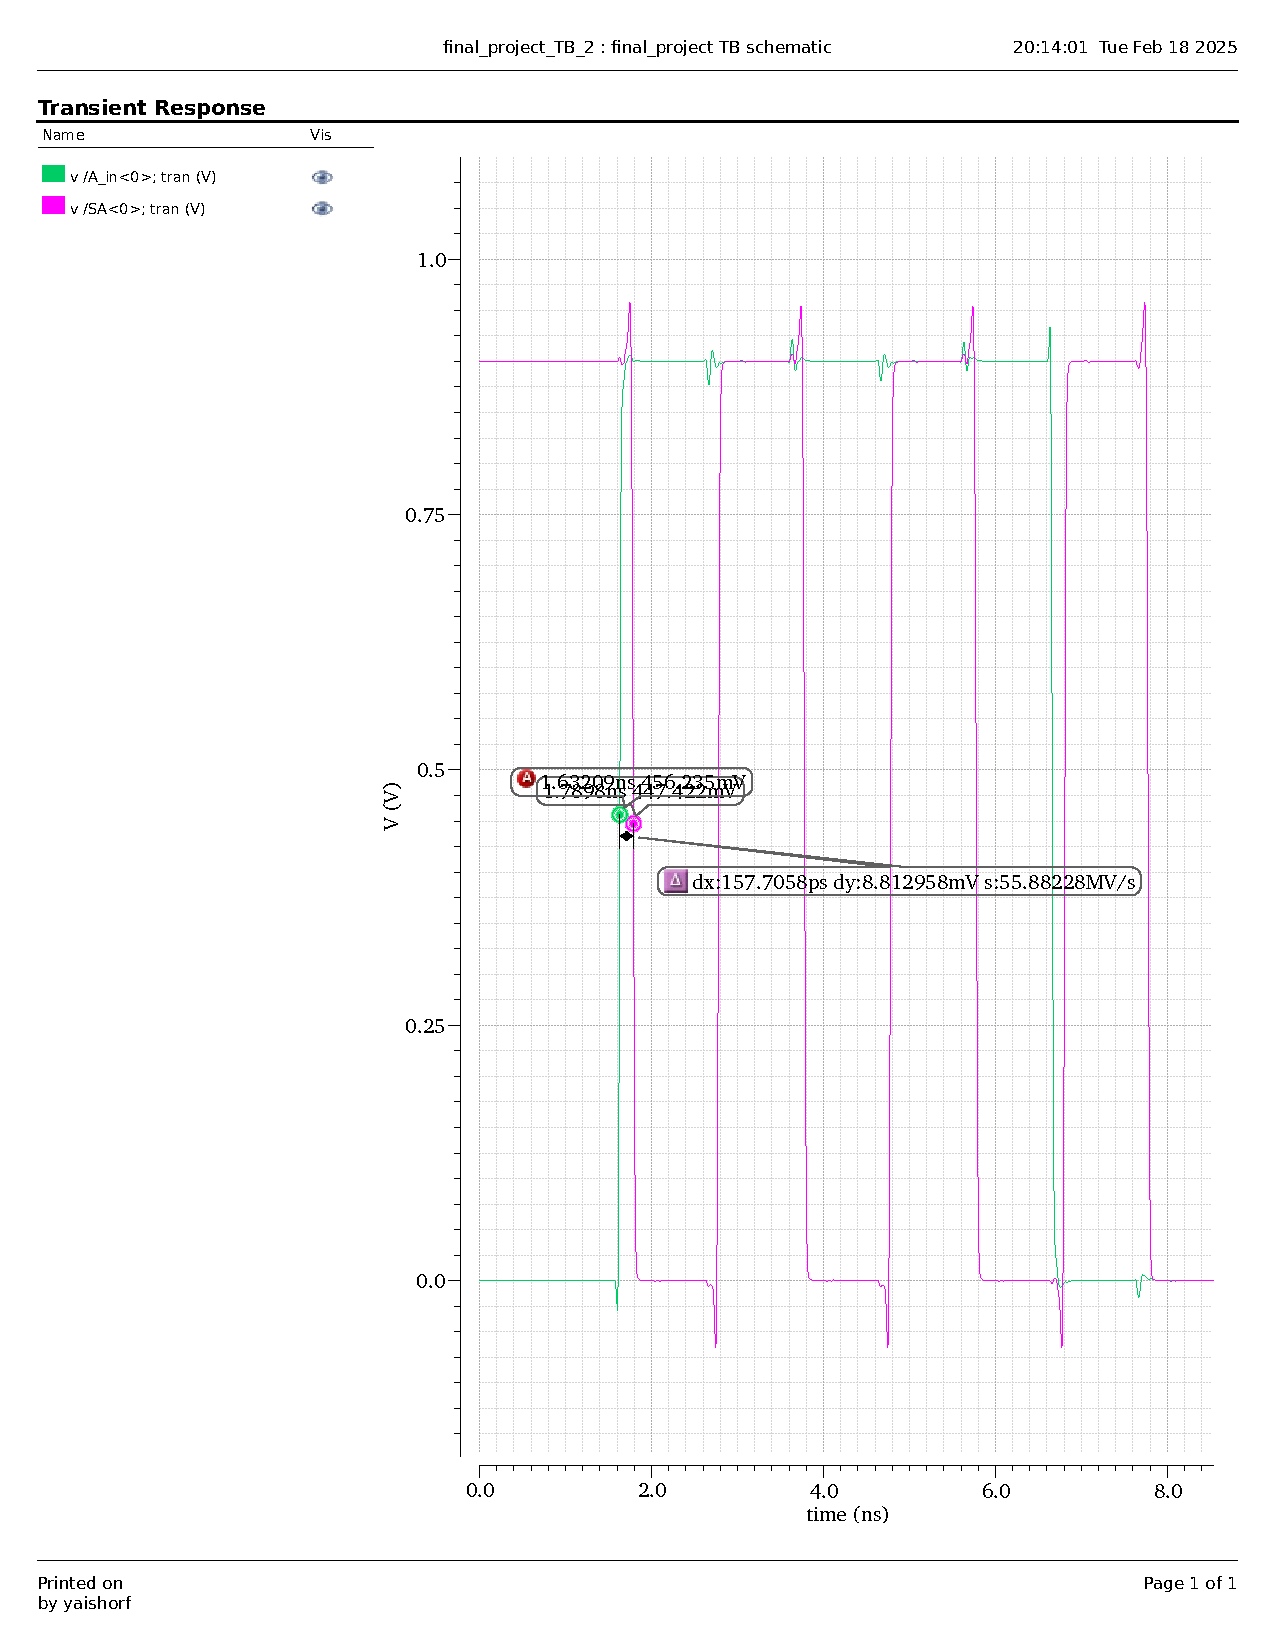
\includegraphics[width=\textwidth]{delay/CP_min_add_0.9_ex.pdf}
        \caption{Minimum delay path - Adder @ 0.9V (After Extraction)}
    \end{minipage}
    \hfill
    \begin{minipage}{0.49\textwidth}
        \centering
        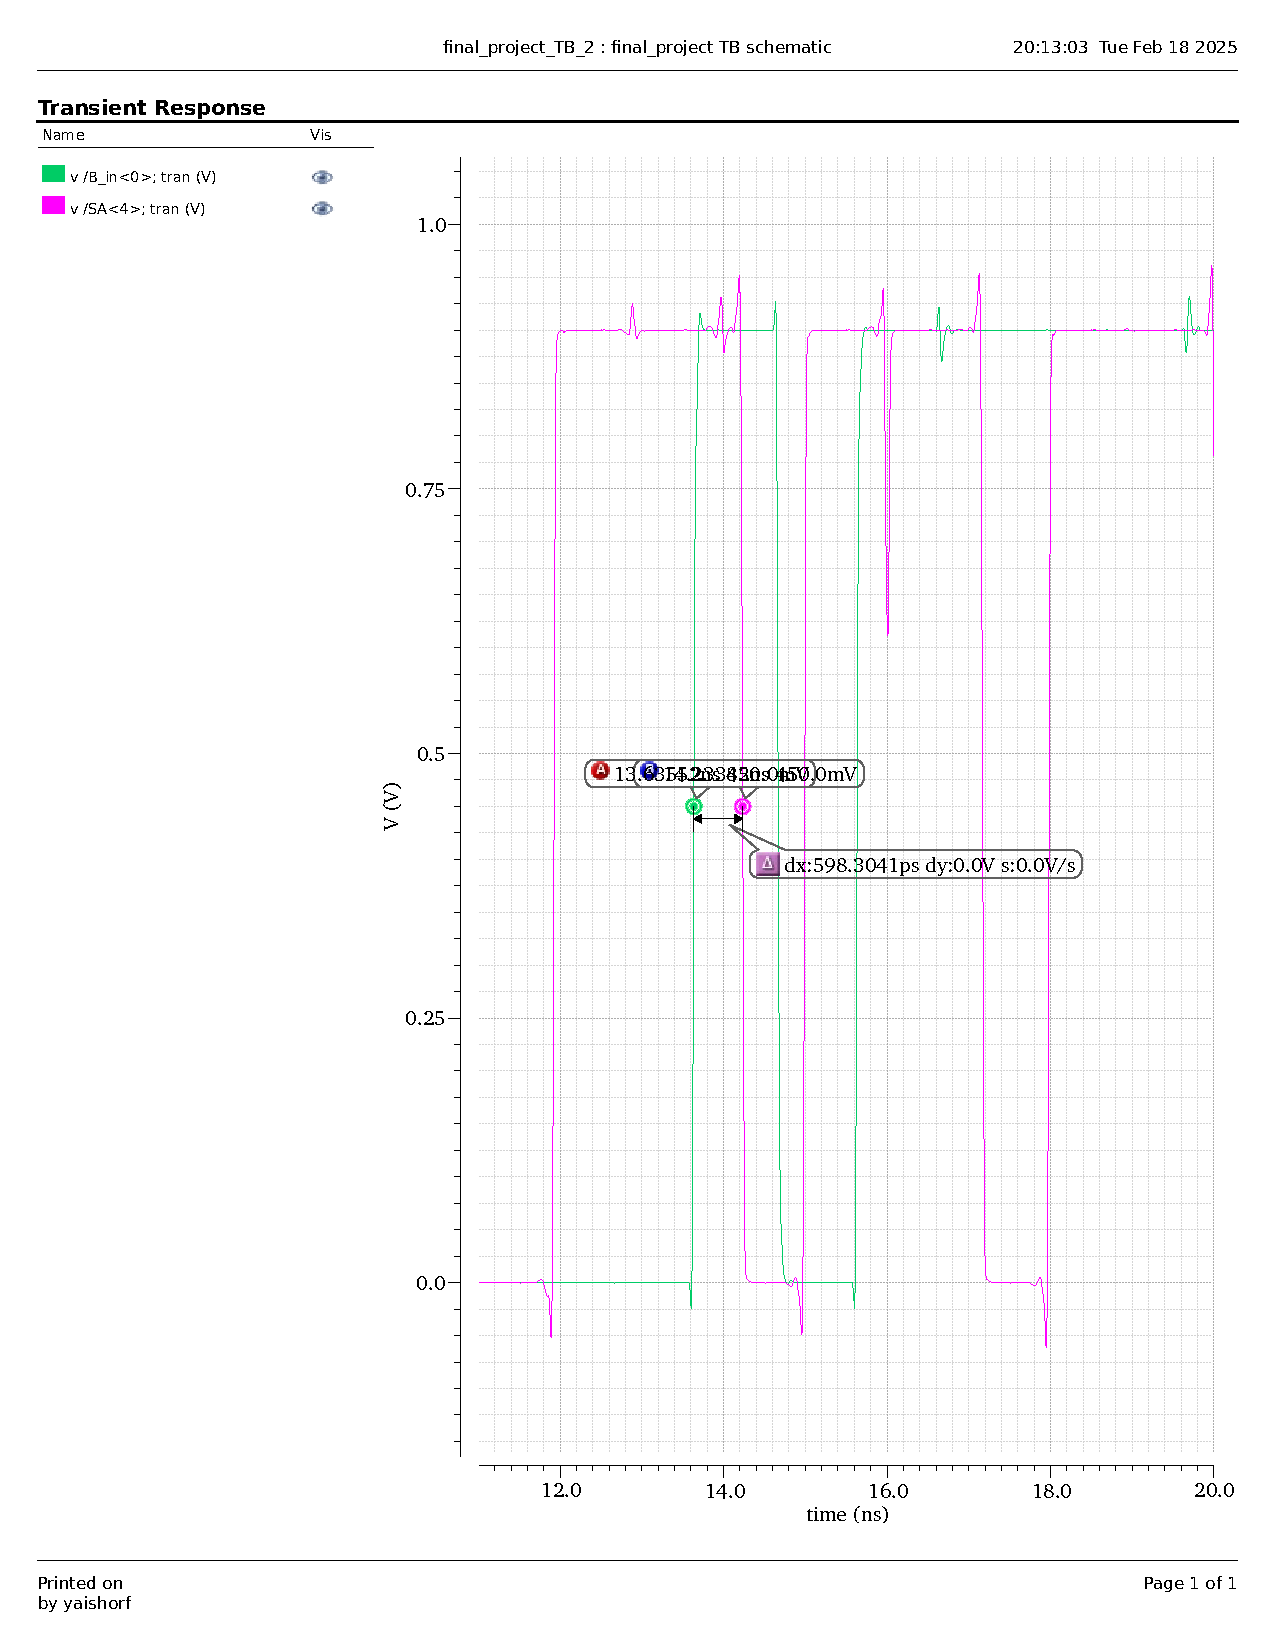
\includegraphics[width=\textwidth]{delay/CP_max_add_0.9_ex.pdf}
        \caption{Maximum delay path - Adder @ 0.9V (After Extraction)}
    \end{minipage}
\end{figure}

\begin{figure}[H]
    \centering
    \begin{minipage}{0.49\textwidth}
        \centering
        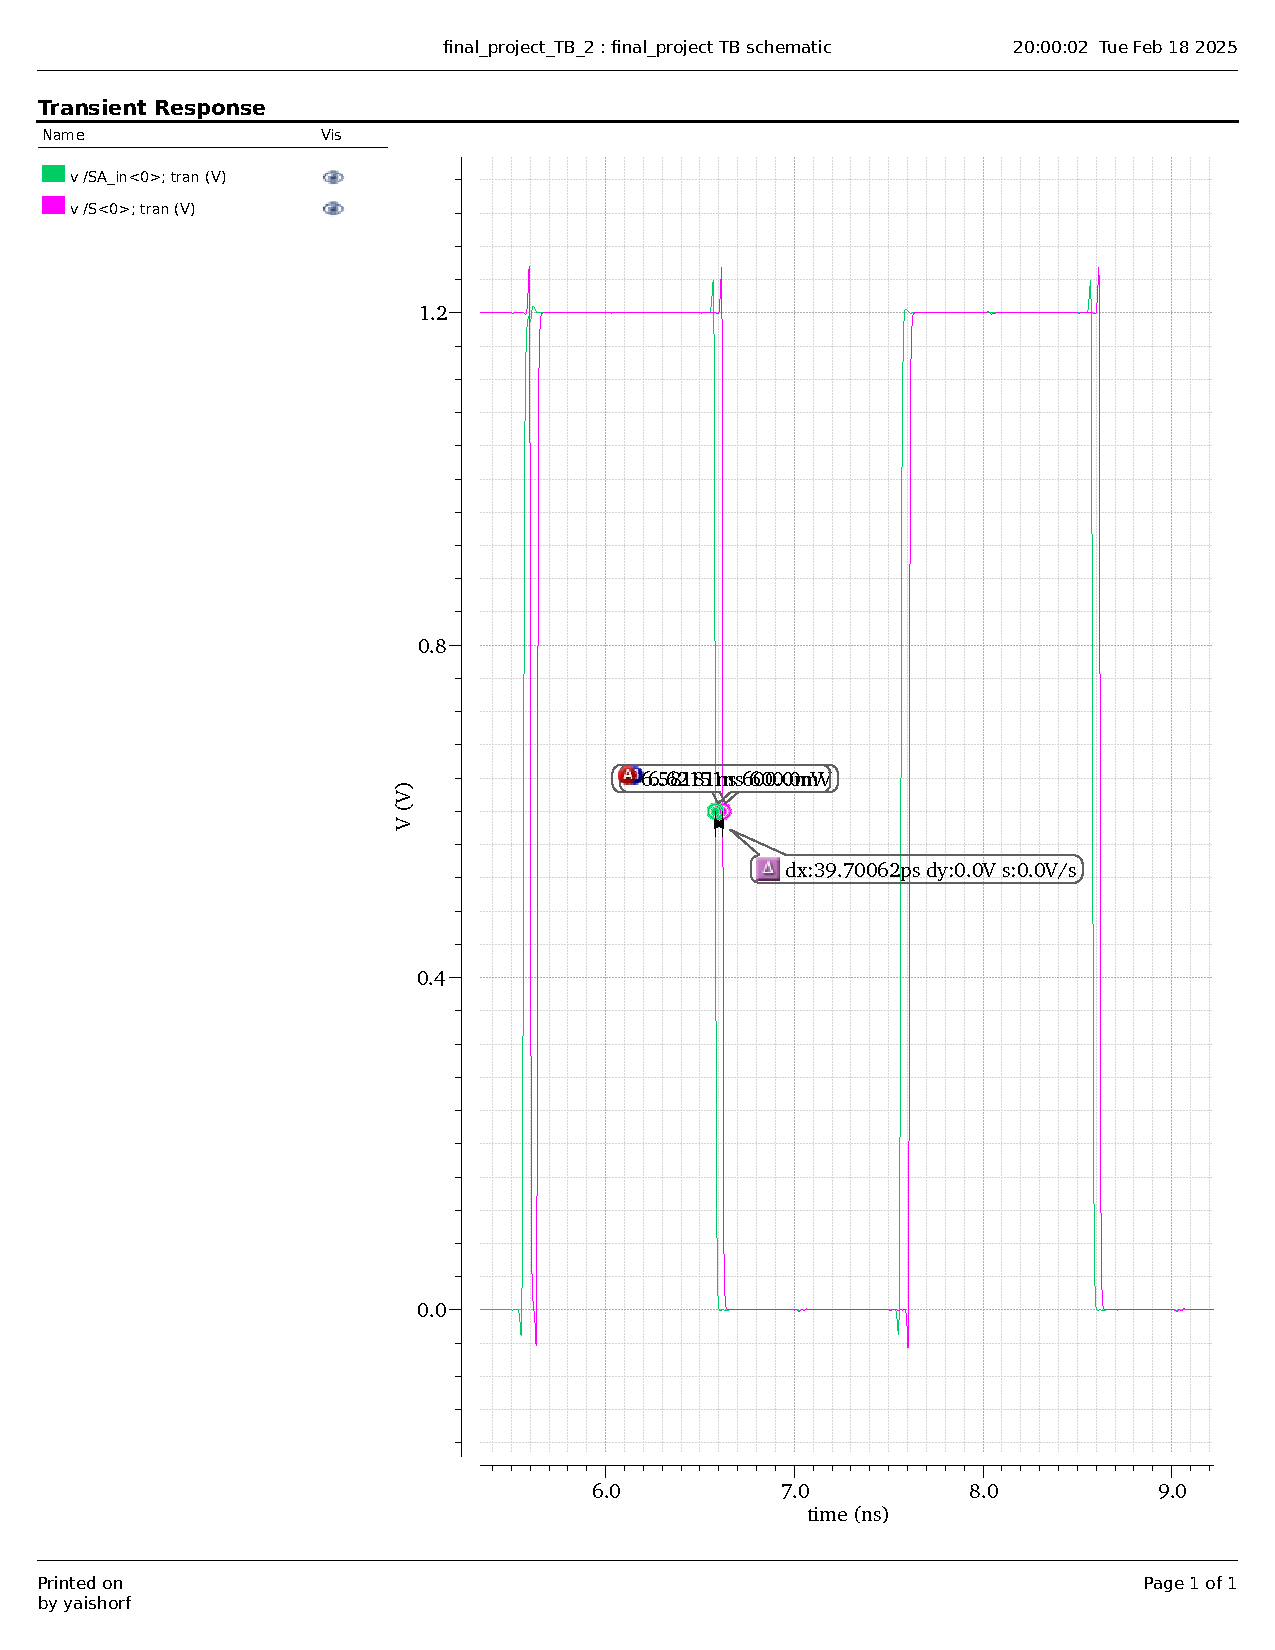
\includegraphics[width=\textwidth]{delay/CP_min_sub_1.2.pdf}
        \caption{Minimum delay path - Subtractor @ 1.2V}
    \end{minipage}
    \hfill
    \begin{minipage}{0.49\textwidth}
        \centering
        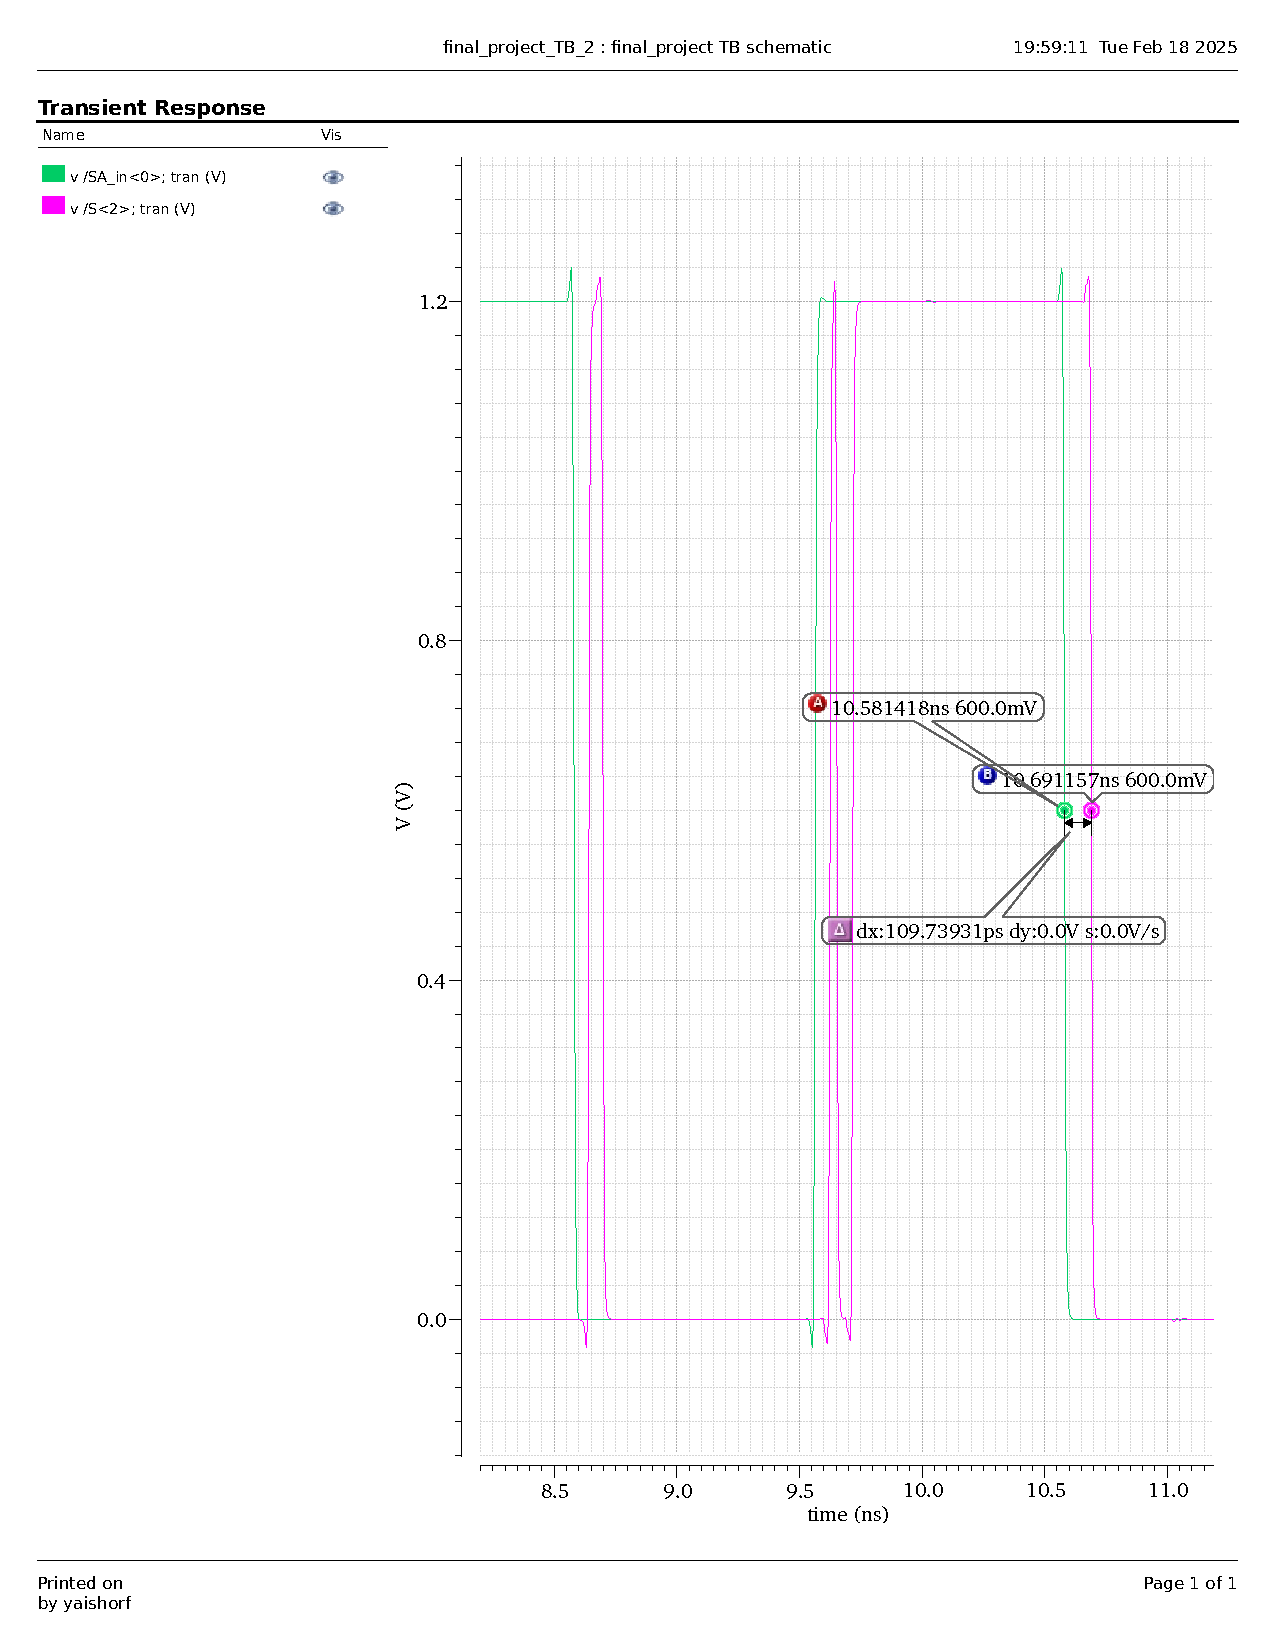
\includegraphics[width=\textwidth]{delay/CP_max_sub_1.2.pdf}
        \caption{Maximum delay path - Subtractor @ 1.2V}
    \end{minipage}
\end{figure}

\begin{figure}[H]
    \centering
    \begin{minipage}{0.49\textwidth}
        \centering
        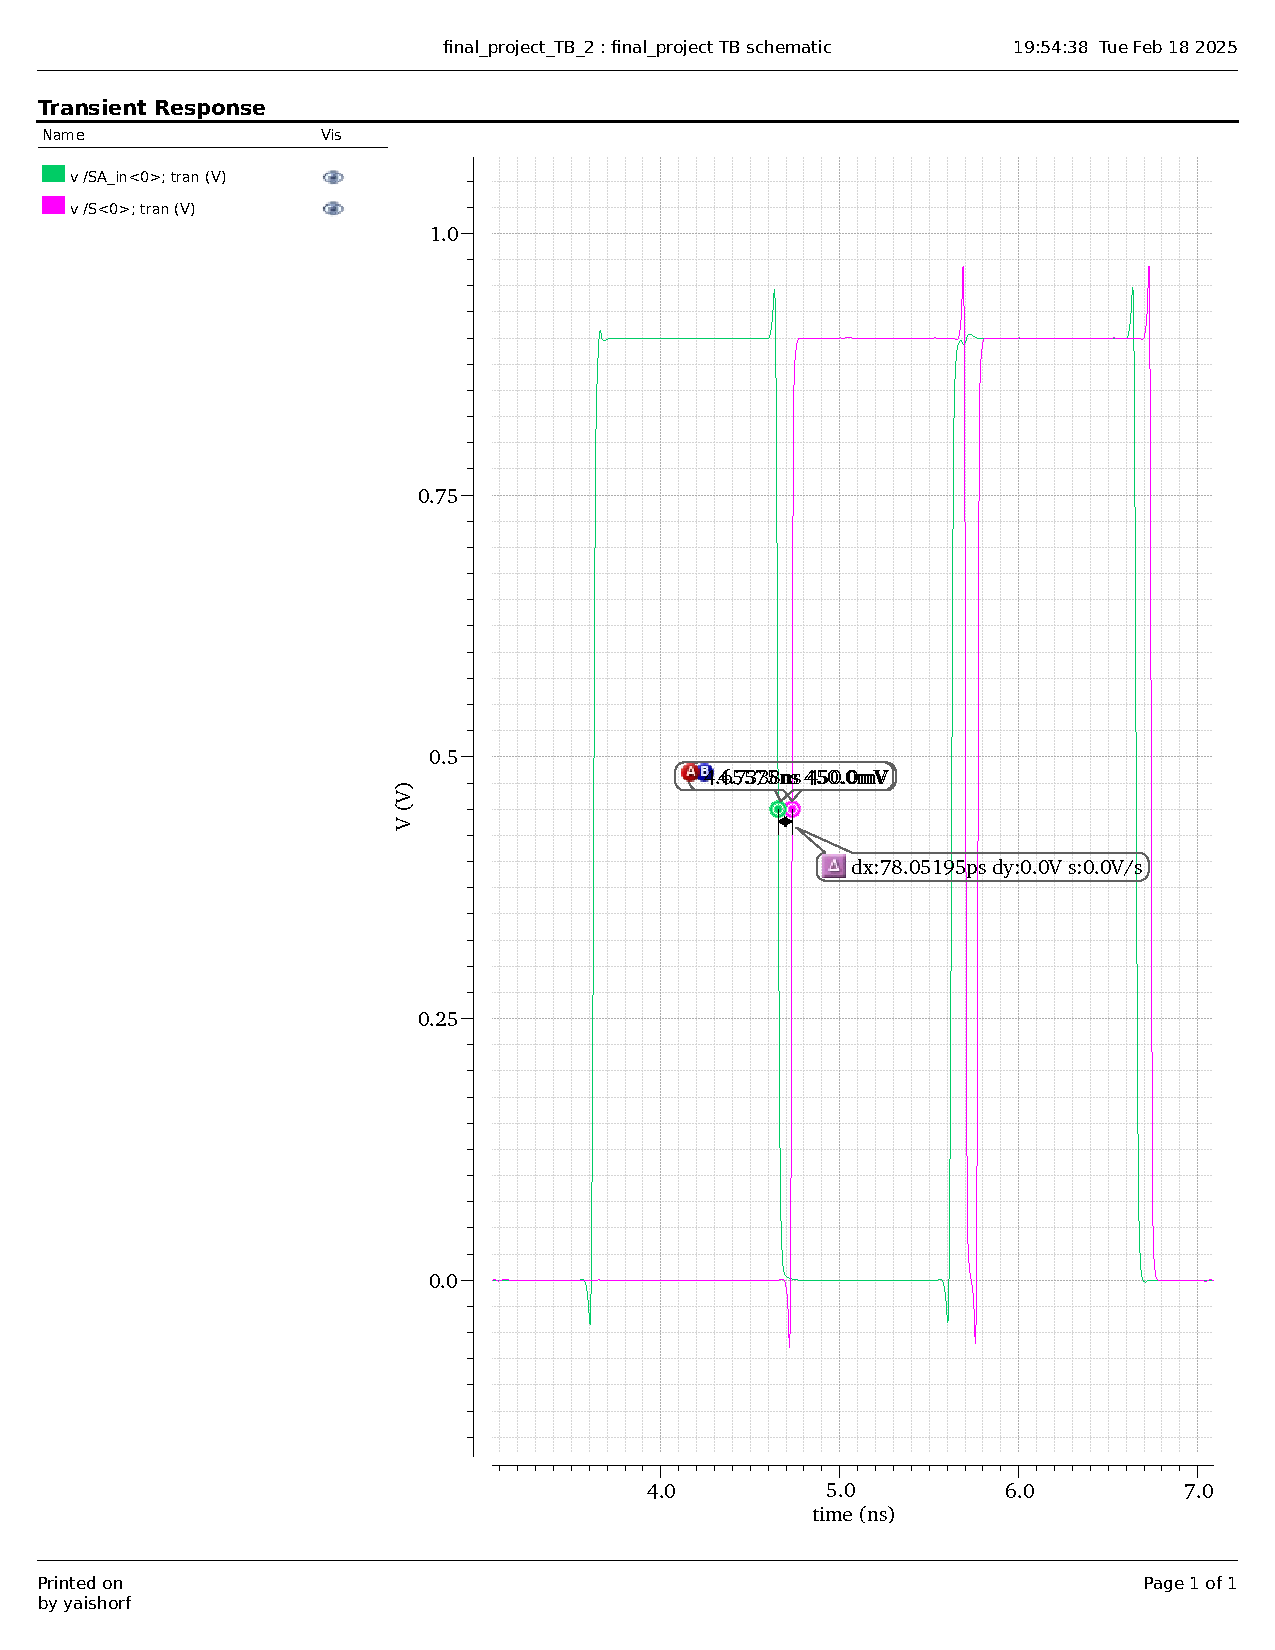
\includegraphics[width=\textwidth]{delay/CP_min_sub_0.9.pdf}
        \caption{Minimum delay path - Subtractor @ 0.9V}
    \end{minipage}
    \hfill
    \begin{minipage}{0.49\textwidth}
        \centering
        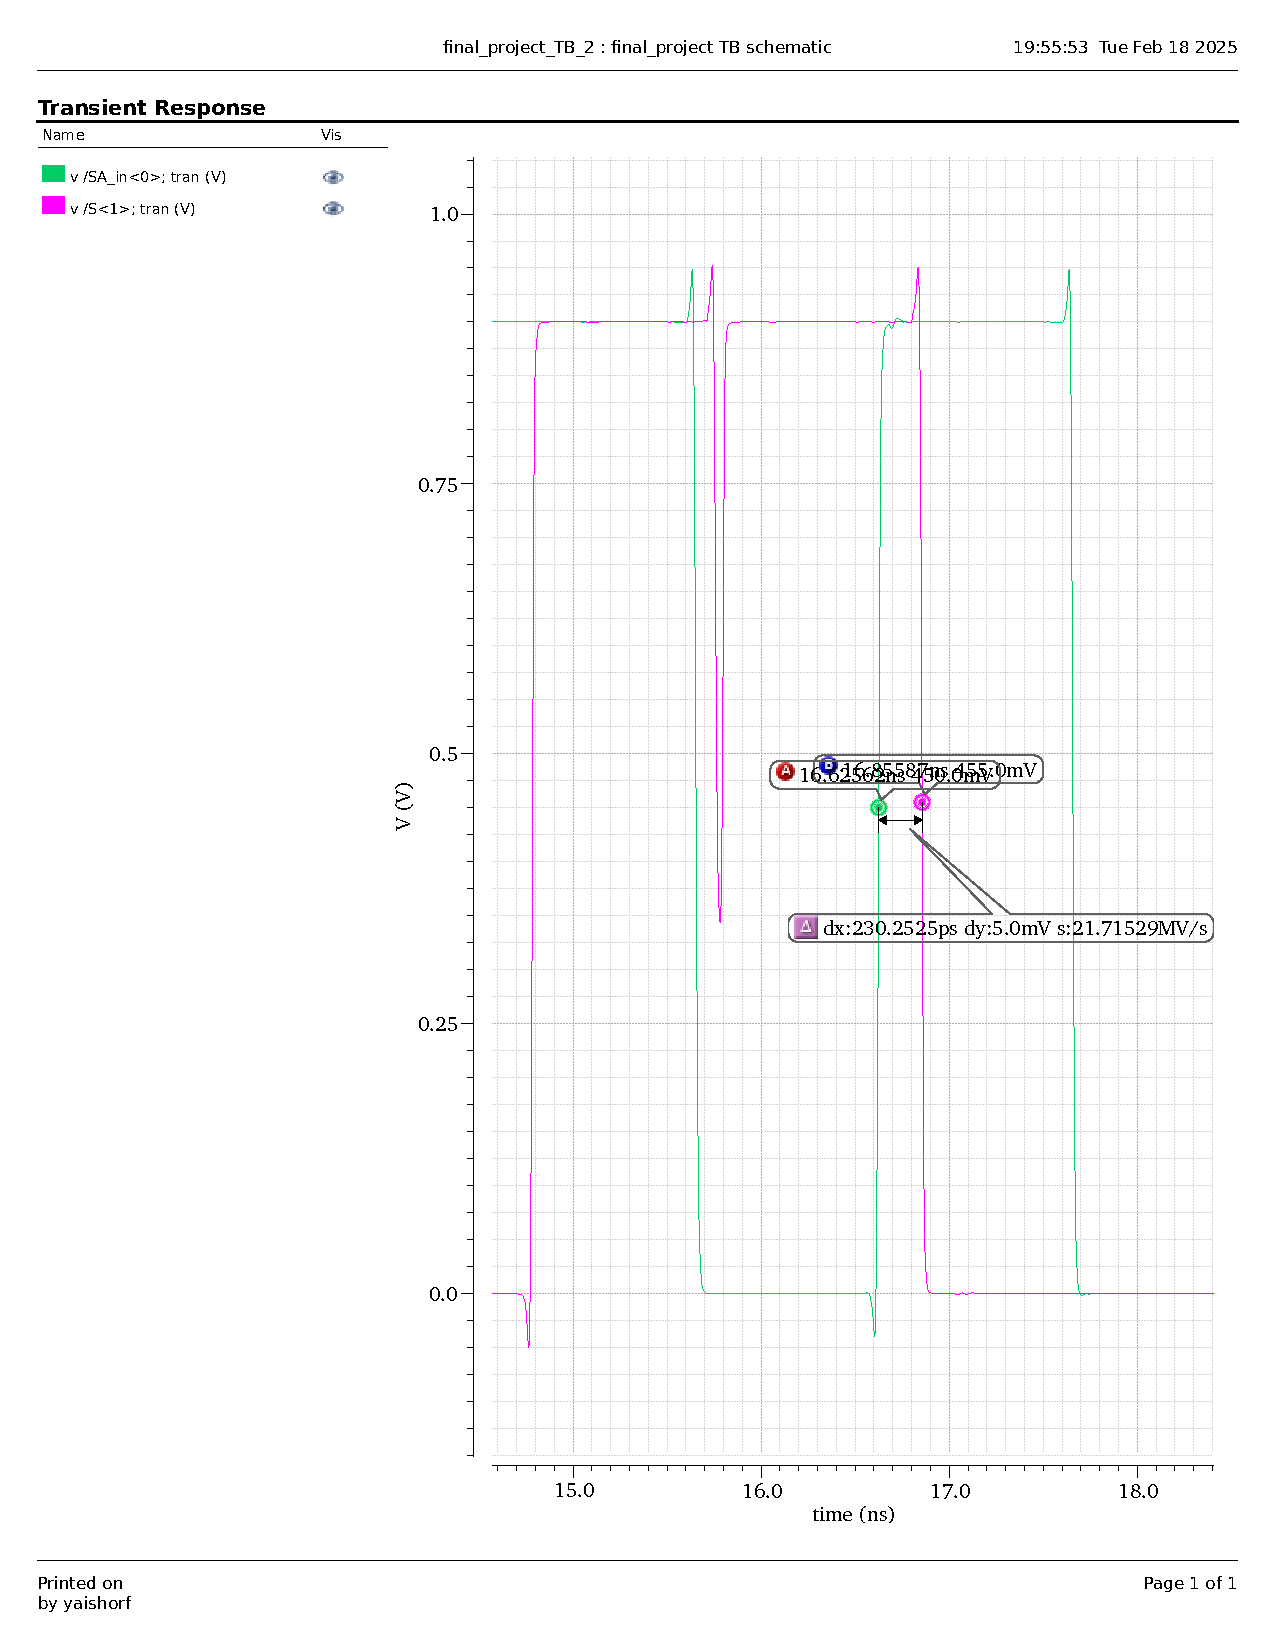
\includegraphics[width=\textwidth]{delay/CP_max_sub_0.9.pdf}
        \caption{Maximum delay path - Subtractor @ 0.9V}
    \end{minipage}
\end{figure}

The results indicate that the extracted circuits exhibit higher delays compared to pre-extraction results due to parasitic effects. The subtractor generally maintains slightly lower delays compared to the adder, which aligns with expectations based on the logical structure.

To further illustrate the critical path analysis, the minimum and maximum delay paths are highlighted in the circuit diagrams. The shortest path is marked in \textbf{green}, while the longest (critical) path is marked in \textbf{red}.

\begin{figure}[H] \centering \begin{minipage}{0.49\textwidth} \centering 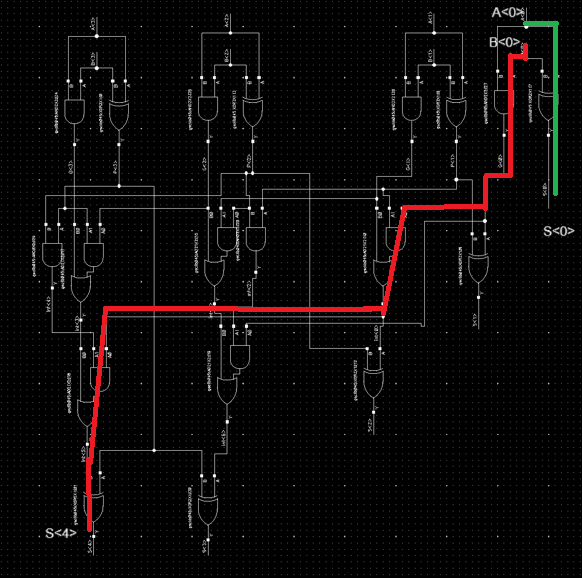
\includegraphics[width=\textwidth]{images/CP_ADD} \caption{Critical path in the adder.} \end{minipage} \hfill \begin{minipage}{0.49\textwidth} \centering 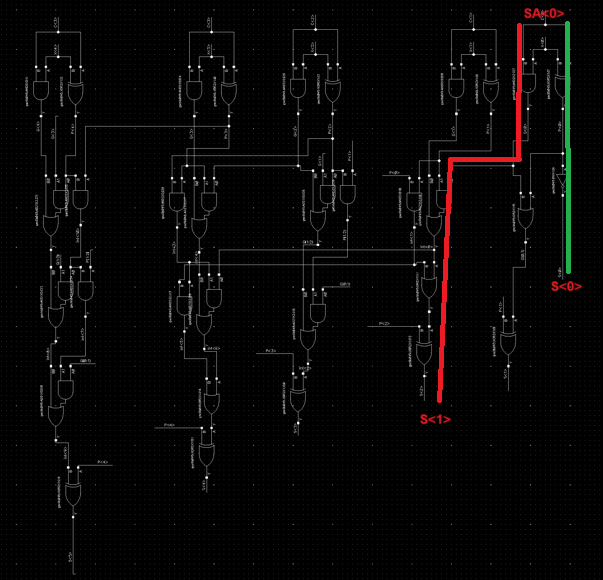
\includegraphics[width=\textwidth]{images/CP_SUB} \caption{Critical path in the subtractor.} \end{minipage} \end{figure}


\subsection{Estimation of Maximum Operating Frequency Based on Hold \& Setup Constraints}

To determine the maximum allowable clock frequency, we analyzed the setup and hold constraints across the different register-to-register paths. The relevant flip-flop delays were obtained for each scenario before and after extraction (EX) and at two operating voltages (0.9V and 1.2V).

The \textbf{FF4} represents the input register to the adder, while \textbf{FF4 \& FF1} correspond to the output of the adder and input to the subtractor, and \textbf{FF4 \& FF2} correspond to the subtractor’s output.

The following constraints were considered:
\begin{itemize}
    \item \textbf{Setup constraint}: The clock period \(T_{clock}\) must be greater than the longest REG-to-REG delay:
    \[
    T_{clock} \geq T_{setup} + T_{CQ} + T_{logic\_max}
    \]
    \item \textbf{Hold constraint}: The hold condition must be satisfied:
    \[
    T_{hold} \geq T_{CQ} + T_{logic\_min}
    \]
    Since \(T_{hold}\) is significantly smaller than the required values, no hold-time violations were observed.
\end{itemize}

The estimated maximum frequency is given by:
\[
f_{max} = \frac{1}{T_{clock}}
\]
where \( T_{clock} \) is derived from the most restrictive delay values across both the adder and subtractor.

\textbf{Calculation:}

For each scenario, we compute the worst-case clock period:

\textbf{Adder Analysis:}

\textbf{Before Extraction (1.2V)}:
\[
T_{clock} = T_{setup} + T_{CQ} + T_{logic\_max}
\]
\[
T_{clock} = 13ps + 62.2ps + 150.8ps = 226ps
\]
\[
f_{max} = \frac{1}{226ps} = 4.42GHz
\]

\textbf{After Extraction (1.2V)}:
\[
T_{clock} = 13ps + 62.2ps + 279.4ps = 354.6ps
\]
\[
f_{max} = \frac{1}{354.6ps} = 2.82GHz
\]

\textbf{Before Extraction (0.9V)}:
\[
T_{clock} = 32ps + 123ps + 336.9ps = 491.9ps
\]
\[
f_{max} = \frac{1}{491.9ps} = 2.03GHz
\]

\textbf{After Extraction (0.9V)}:
\[
T_{clock} = 32ps + 123ps + 598.8ps = 753.8ps
\]
\[
f_{max} = \frac{1}{753.8ps} = 1.33GHz
\]

\textbf{Subtractor Analysis:}

\textbf{Before Extraction (1.2V)}:
\[
T_{clock} = 15ps + 52ps + 114.2ps = 181.2ps
\]
\[
f_{max} = \frac{1}{181.2ps} = 5.52GHz
\]

\textbf{After Extraction (1.2V)}:
\[
T_{clock} = 15ps + 52ps + 279.4ps = 346.4ps
\]
\[
f_{max} = \frac{1}{346.4ps} = 2.89GHz
\]

\textbf{Before Extraction (0.9V)}:
\[
T_{clock} = 36ps + 104ps + 162.2ps = 302.2ps
\]
\[
f_{max} = \frac{1}{302.2ps} = 3.31GHz
\]

\textbf{After Extraction (0.9V)}:
\[
T_{clock} = 36ps + 104ps + 598.8ps = 738.8ps
\]
\[
f_{max} = \frac{1}{738.8ps} = 1.35GHz
\]

\textbf{Final Operating Frequency Selection:}

The final maximum frequency must be the lowest common frequency that satisfies both the adder and subtractor constraints.

\begin{table}[H]
    \centering
    \begin{tabular}{|c|c|c|}
        \hline
        Condition & Voltage & Final \( f_{max} \) (GHz) \\
        \hline
        Before EX & 1.2V & 4.42 \\
        After EX & 1.2V & 2.82 \\
        Before EX & 0.9V & 2.97 \\
        After EX & 0.9V & 1.35 \\
        \hline
    \end{tabular}
    \caption{Final maximum operating frequency selection}
\end{table}


\subsection{Verification of Maximum Operating Frequency}

To ensure the circuit's correctness at the estimated maximum operating frequency, two key aspects were examined: 
\begin{itemize}
    \item \textbf{Logical correctness}: Verifying that after two clock cycles from the input application, the expected output is correctly produced.
    \item \textbf{Transition time validation}: Ensuring that the transition times (rise and fall) remain within acceptable limits.
\end{itemize}

To efficiently verify transition times across all signals in both the adder and subtractor, a custom script was used to measure rise and fall times. The following is a characteristic output from the script:
\begin{figure}[H]
    \centering
    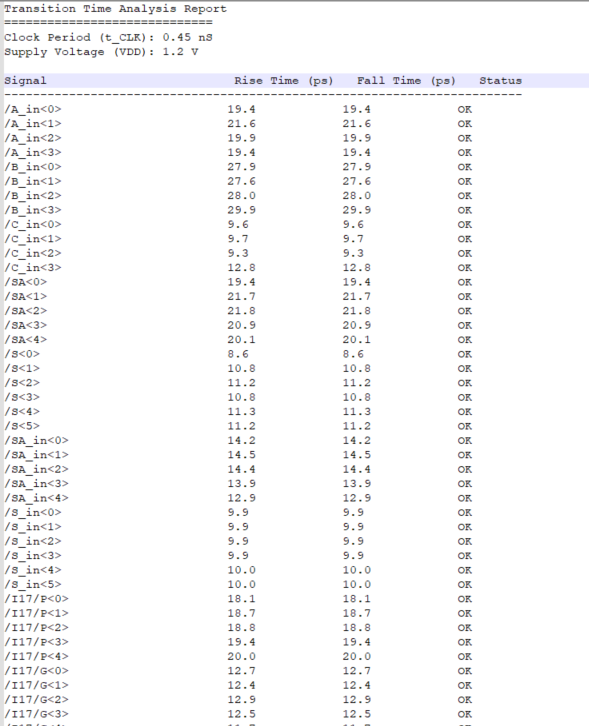
\includegraphics[width=0.8\textwidth]{min_freq_af_ex_1.2/Transition_Times_0.45nS_1.2V.png}
    \caption{Measured transition times at 1.2V after extraction.}
\end{figure}

As expected, the actual operating frequency was slightly lower than the initially estimated values.

\begin{table}[H]
    \centering
    \begin{tabular}{|c|c|c|c|}
        \hline
        Voltage & Estimated Period (ps) & Verified Period (ps) & Max Transition Time (ps) \\
        \hline
 1.2V (Before EX) & 226 & 300 & 14.2 \\
        0.9V (Before EX) & 491.9 & 600 & 32.0 \\
        1.2V (After EX) & 354.6 & 450 & 30.0 \\
        0.9V (After EX) & 753.8 & 800 & 46.9 \\
        \hline
    \end{tabular}
    \caption{Comparison of Estimated vs. Verified Maximum Operating Frequency}
\end{table}

The results confirm that the transition times increase with lower supply voltages and after extraction due to additional parasitics. Despite the small deviation from the expected values, the circuit remains within acceptable operating limits.


\section{Conclusions}
This project successfully demonstrated the design and implementation of a \textbf{4-bit ALU} using \textbf{gpdk045/gsclib045} technology. The final implementation met all the original design requirements: the circuit area remained within the allowed limits (\textbf{56.29 $\mu m^2$} compared to the \textbf{82.32 $\mu m^2$} constraint), rise and fall times were kept below \textbf{50ps}, and the circuit operated correctly under both required supply voltages (\textbf{0.9V and 1.2V}).

The use of the \textbf{Knowles adder} enabled an efficient balance between speed and power consumption, achieving a maximum operating frequency of \textbf{2.82GHz} at \textbf{1.2V} and \textbf{1.35GHz} at \textbf{0.9V} after the extraction process. The most significant challenge was the \textbf{layout design}, which required careful optimization of component placement and wiring paths to meet area constraints while maintaining optimal performance.

For future improvements, further optimizations in cell placement and wiring design could be explored to reduce delays and improve circuit density.

\section{References}
\begin{itemize}
    \item Weste, Neil, and David Harris. "CMOS VLSI Design: A Circuits and Systems Perspective." 4th ed. Addison-Wesley, 2010.
\end{itemize}

\end{document}
